\chapter{Diseño del Sistema}

\section{Diseño de la arquitectura del sistema}
Establecer el ámbito de las tareas que realiza la API, es el primer paso para conseguir un buen diseño de la arquitectura. Conocer a priori en qué momento se ejecutan cada una, es lo que ayuda a clasificarlas de alguna manera. Dicho esto, se pensó que lo mejor era dividir el programa se divide en tres niveles o capas, superior o de interfaz, intermedia o de comunicación, e inferior o de procesamiento, como se puede apreciar en la figura \ref{fig:arquitecturadelsistema}. 

\begin{figure}
	\centering
	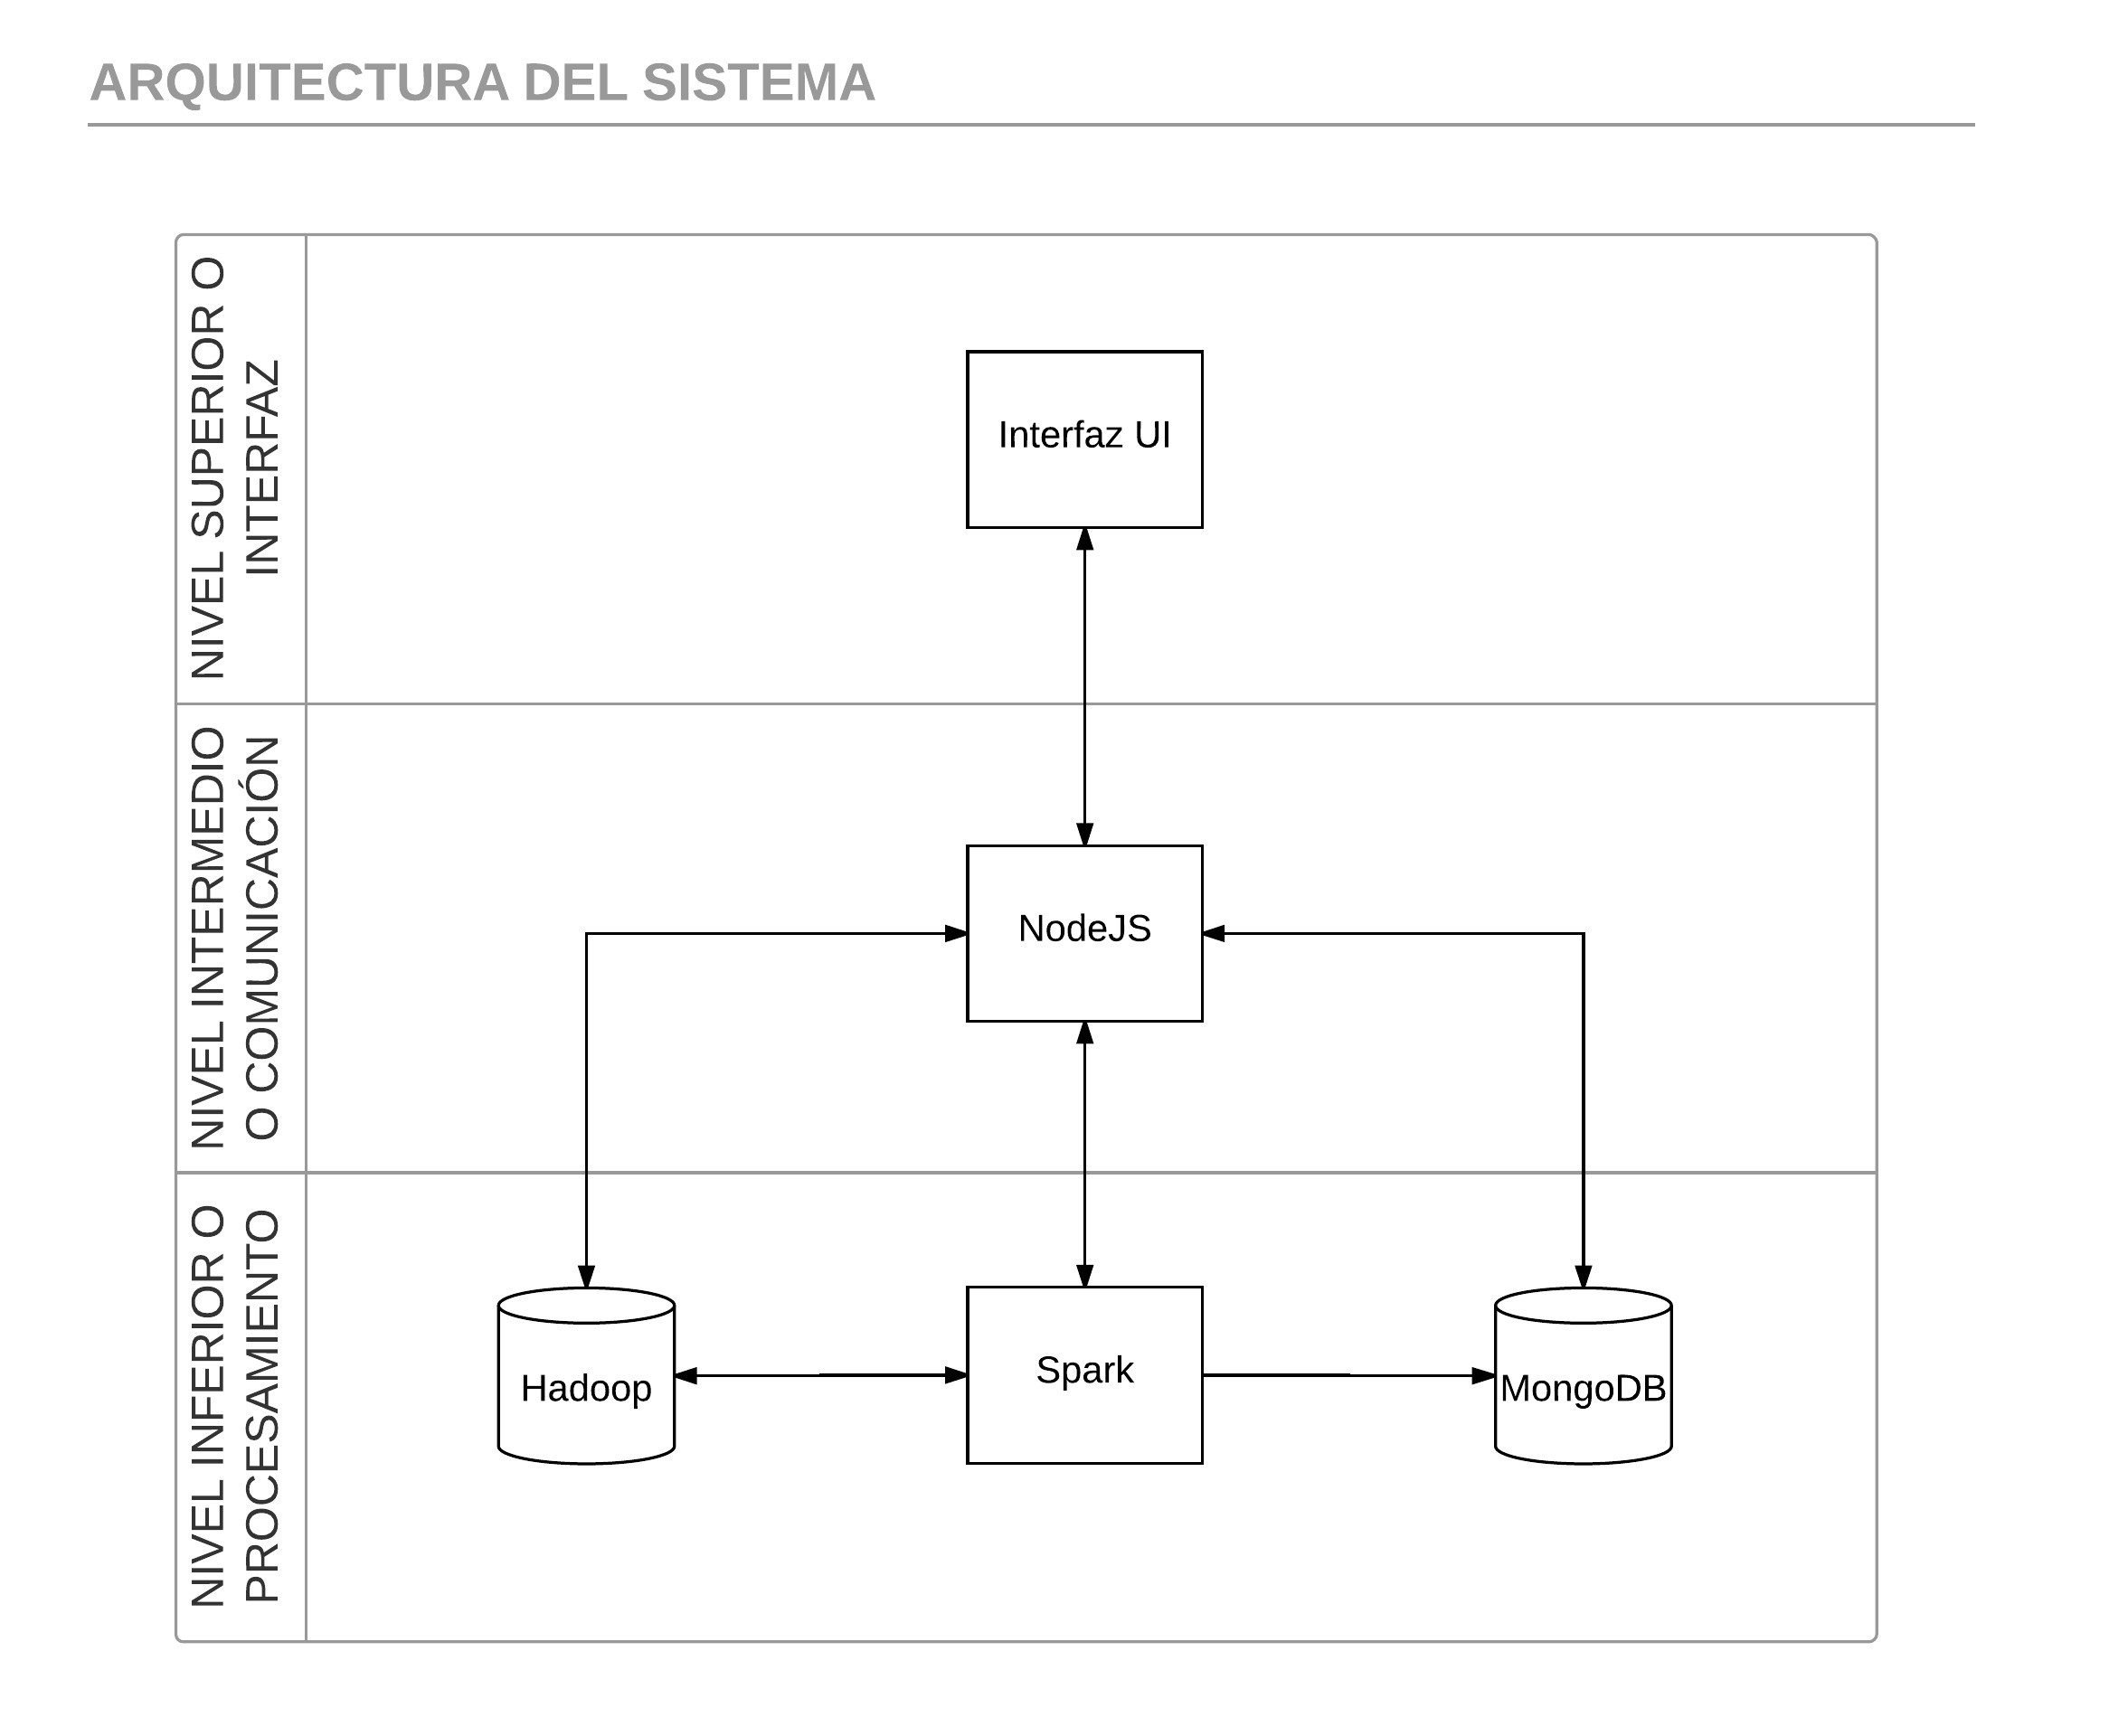
\includegraphics[width=1\linewidth]{imagenes/Arquitectura_del_sistema}
	\caption{Diseño de la arquitectura del sistema}
	\label{fig:arquitecturadelsistema}
\end{figure}

El nivel superior o nivel de interfaz, es el encargado de comunicarse directamente con el usuario de la aplicación. En él, se aloja la parte web con la que trabajan los usuarios, permitiendo recoger la información que solicitan, para después, enviarla al nivel intermedio. La interfaz de la API está diseñada para poder trabajar con varios usuarios de manera concurrente, o poder trabajar sobre varias pestañas o ventanas una sola persona. Toda la funcionalidad de esta capa está escrita en Javascript, haciendo que la interfaz sea dinámica. Como se pudo ver en el capítulo anterior, la figura \ref{fig:interfazinicial} muestra el diseño de esta interfaz.

En el nivel intermedio o de comunicación, es donde se realiza toda la comunicación entre las distintas herramientas y hace que el flujo de datos entre la capa superior y la inferior sea el correcto. Aquí es donde se ejecuta NodeJS, siendo el encargado de recoger todos los tipos de eventos y acciones que se producen en la capa superior, para a continuación, realizar la solicitud de procesamiento de la información recibida a la capa inferior donde se encuentra Spark. Se puede decir que es el corazón del sistema, donde se gestiona toda la información y también es el encargado de crear el servidor virtual permitiendo que la aplicación pueda funcionar a través de un navegador web. 
También se encarga de la comunicación con MongoDB para obtener los resultados devueltos por Spark, para a continuación, dibujar el gráfico solicitado y después mandarlo a la capa superior, utilizando para ello la librería D3JS. 

Por último, en el nivel inferior o de procesamiento, se aplican los esquemas de agrupación y las técnicas de reducción elegidas para cada uno de los gráficos disponibles en la API. En este nivel es donde se alojan las herramientas Hadoop, Spark y MongoDB. Cada una de ellas tiene su propia función dentro del nivel, siendo así Hadoop el encargado de almacenar y mantener los datos del sistema, Spark el encargado de coger el fichero del HDFS, procesando los datos aplicando los esquemas de agrupación y las técnicas de reducción elegidas para cada uno de los gráficos disponibles en la API, y por parte de MongoDB, guardar el resultado enviado del procesado de Spark, manteniendo información acerca del estado de cada uno de los resultados, como la fecha de inicio de solicitud, o la de finalizado el cálculo, además de información acerca de si se está ejecutando en un instante preciso o ha finalizado. Esto ayuda para conocer si se está procesando ya un gráfico con unos parámetros y fichero de datos concreto, y se vuelve a solicitar, no volver a realizar el cálculo, sino esperar a que ese termine para devolver el resultado a la capa de comunicación.

\section{Conexión entre módulos}
En esta sección se va a explicar cómo se han conectado cada uno de los diferentes módulos o programas para que puedan comunicarse entre sí y que realicen su función de manera autónoma. Para ello, se va a dividir y explicar cada una de las conexiones. Algunos de las librerías que se utilizan para conectar los sistemas, deben añadirse con ayuda del gestor de paquetes ‘Sbt’ para poder utilizarlo en el código, y en el caso de NodeJS, se utiliza el gestor ‘NPM’.

\subsection{Hadoop - Spark}
La conexión entre estas dos herramientas viene integrada en el propio Spark. Es tan sencillo como crear el sqlContext a partir del SparkConfig, que viene en el paquete ‘Spark-sql’ y utilizar el método ‘read’ que trae la propia aplicación, pasándole como parámetro la URL donde se aloja el fichero en el HDFS. En la figura \ref{fig:conexionhadoopspark}, se muestra el flujo de llamadas entre las dos herramientas.

\begin{figure}
	\centering
	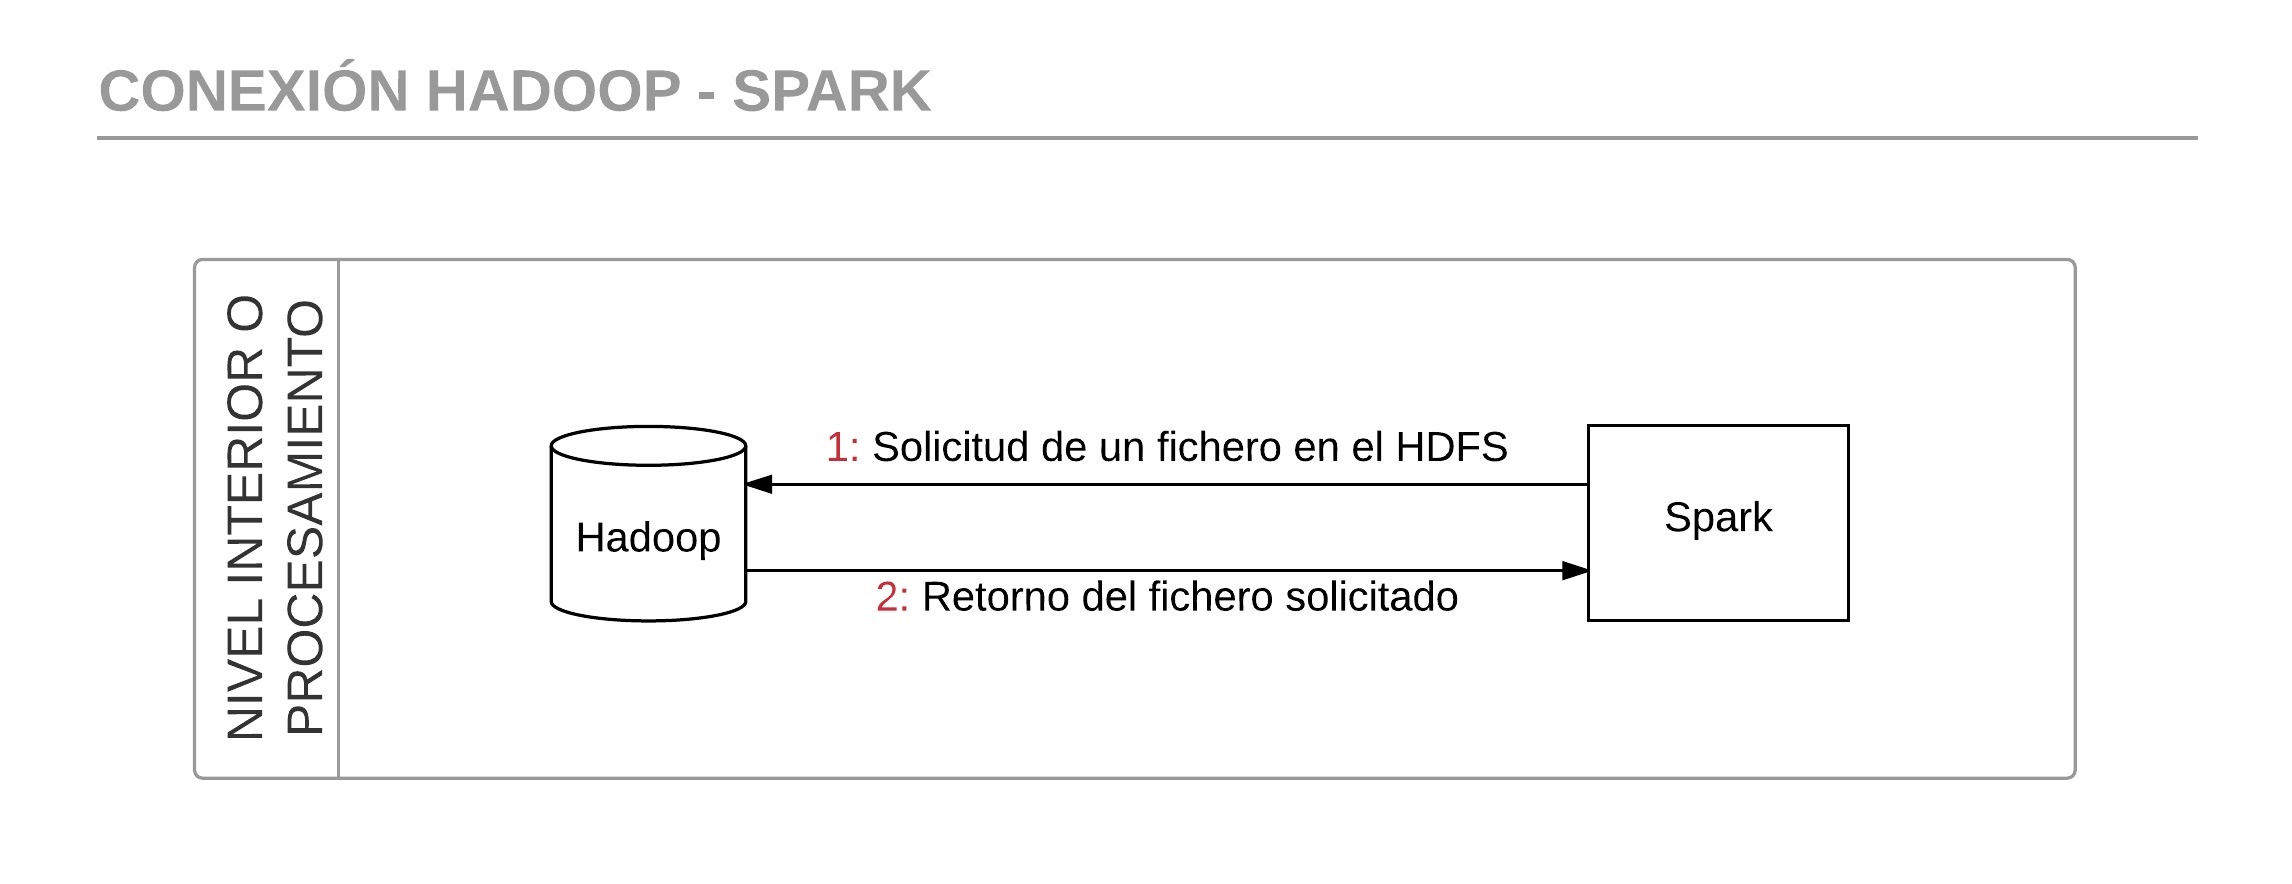
\includegraphics[width=1\linewidth]{imagenes/Conexion_Hadoop_Spark}
	\caption{Representación gráfica de la conexión Hadoop - Spark}
	\label{fig:conexionhadoopspark}
\end{figure}

\subsection{Spark - MongoDB}
Spark no trae integrada la conexión con MongoDB como ocurre en el caso de Hadoop. Para ello, la empresa de MongoDB provee una librería llamada ‘Mongo-Spark-Connector’ \cite{SparkMongoConexion}, que contiene las funciones necesarias para establecer comunicación entre estas dos herramientas. 

\begin{figure}
	\centering
	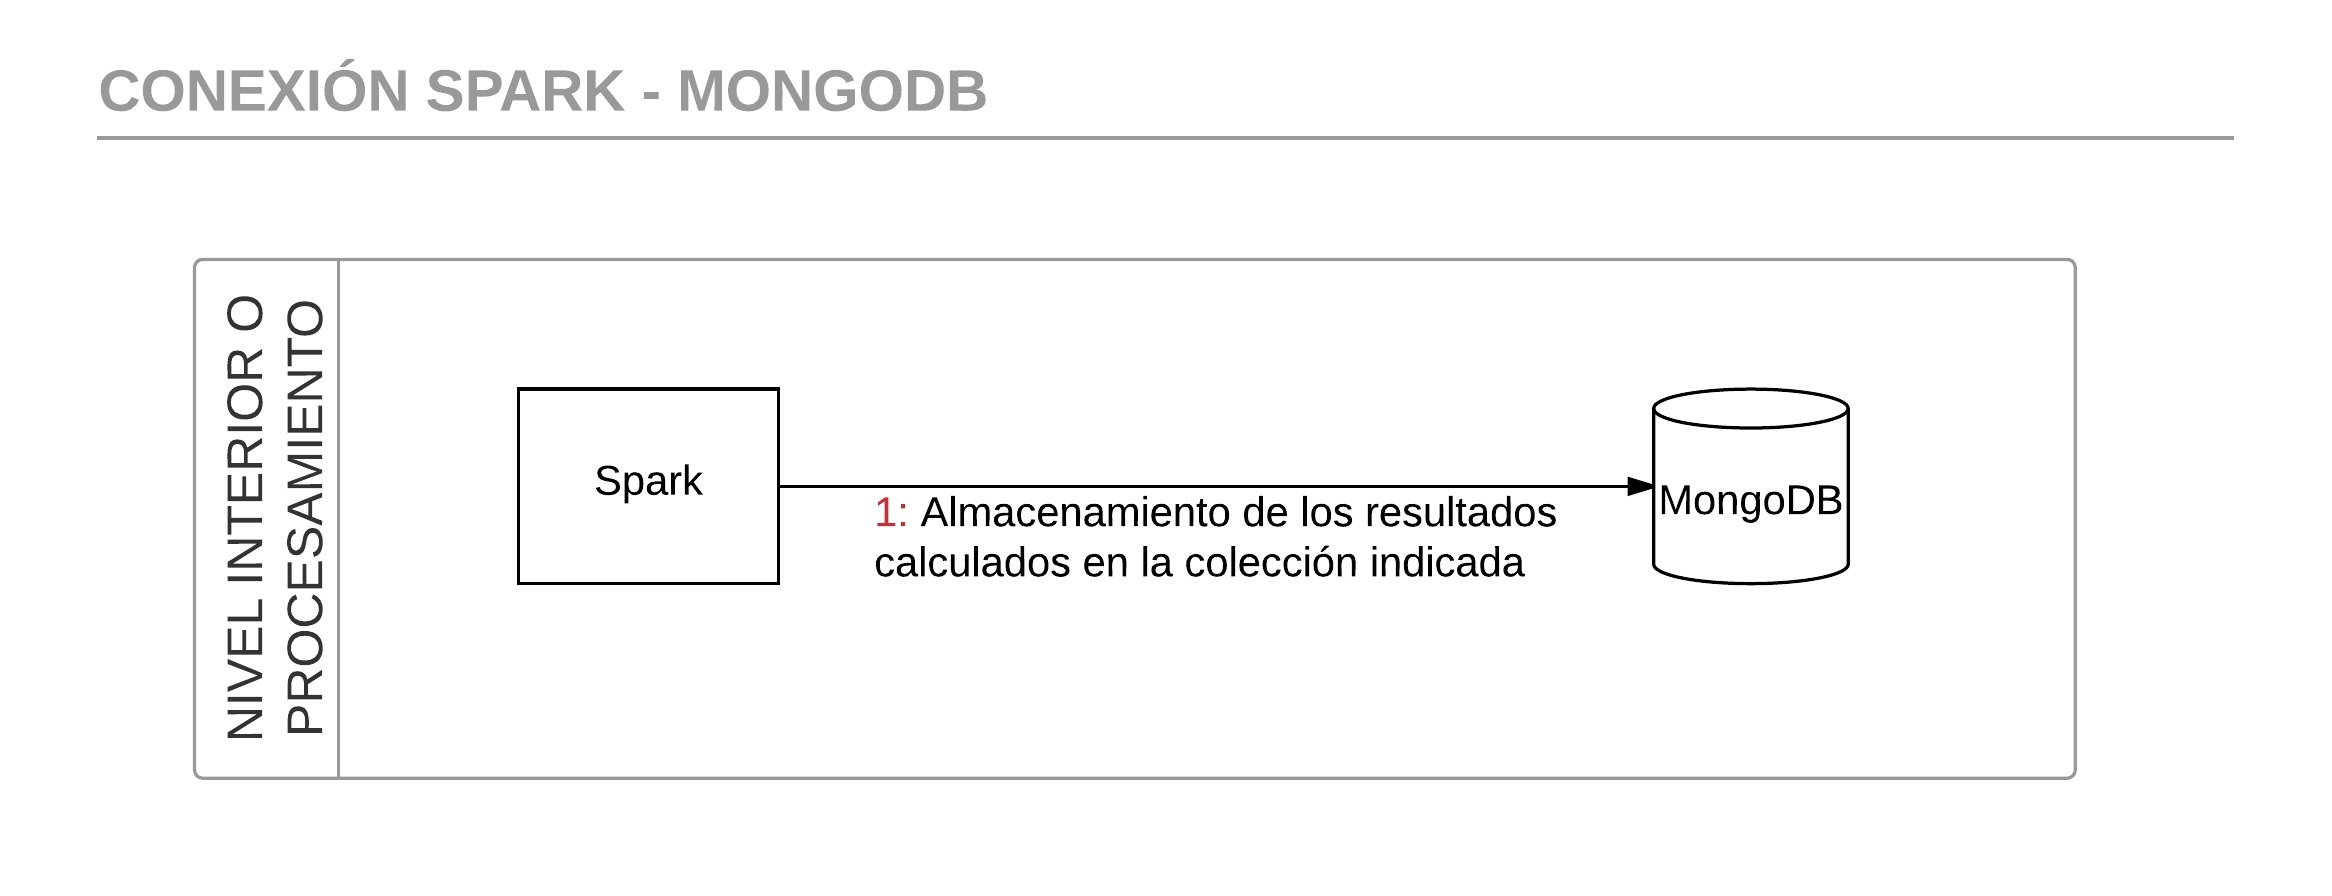
\includegraphics[width=1\linewidth]{imagenes/Conexion_Spark_MongoDB}
	\caption{Representación gráfica de la conexión Spark - MongoDB}
	\label{fig:conexionsparkmongodb}
\end{figure}

Conociendo la URL donde está mongo activo, la base de datos y la colección donde se quiere almacenar el resultado generado y el SparkContext, es suficiente para utilizar el método ‘WriteConfig’ que provee esta librería. Después, pasando el resultado a una estructura de secuencia de Spark y posteriormente a JSON, se guarda el mismo utilizando la función ‘save’ de ‘MongoSpark’. Con esto, ya estaría el resultado en MongoDB a través de Spark. En la figura \ref{fig:conexionsparkmongodb} se aprecia el flujo de almacenamiento de los datos resultados.

\subsection{NodeJS - Hadoop}
Para obtener el listado de los ficheros y directorios dentro de una URL específica, la mejor forma es utilizar la API RESTful \cite{HadoopRestful} que proporciona Hadoop. Para ello es necesario utilizar la librería ‘Request’ de NodeJS, que permite realizar peticiones de tipo ‘get’ o ‘post’ a una URL de una web, pudiendo guardar el resultado en una variable. Solamente indicando la dirección y el puerto que da Hadoop para la API RESTful, indicándole la ruta donde se encuentra el archivo dentro del HDFS, y la opción ‘?op=LISTSTATUS’, se obtiene el resultado de una manera muy rápida, como se muestra en la figura \ref{fig:conexionnodejshadoop}. En este caso, en vez de guardarla, se redirecciona a la interfaz web para poder visualizarla. Después se le da formato en la interfaz con funciones Javascript.

\begin{figure}
	\centering
	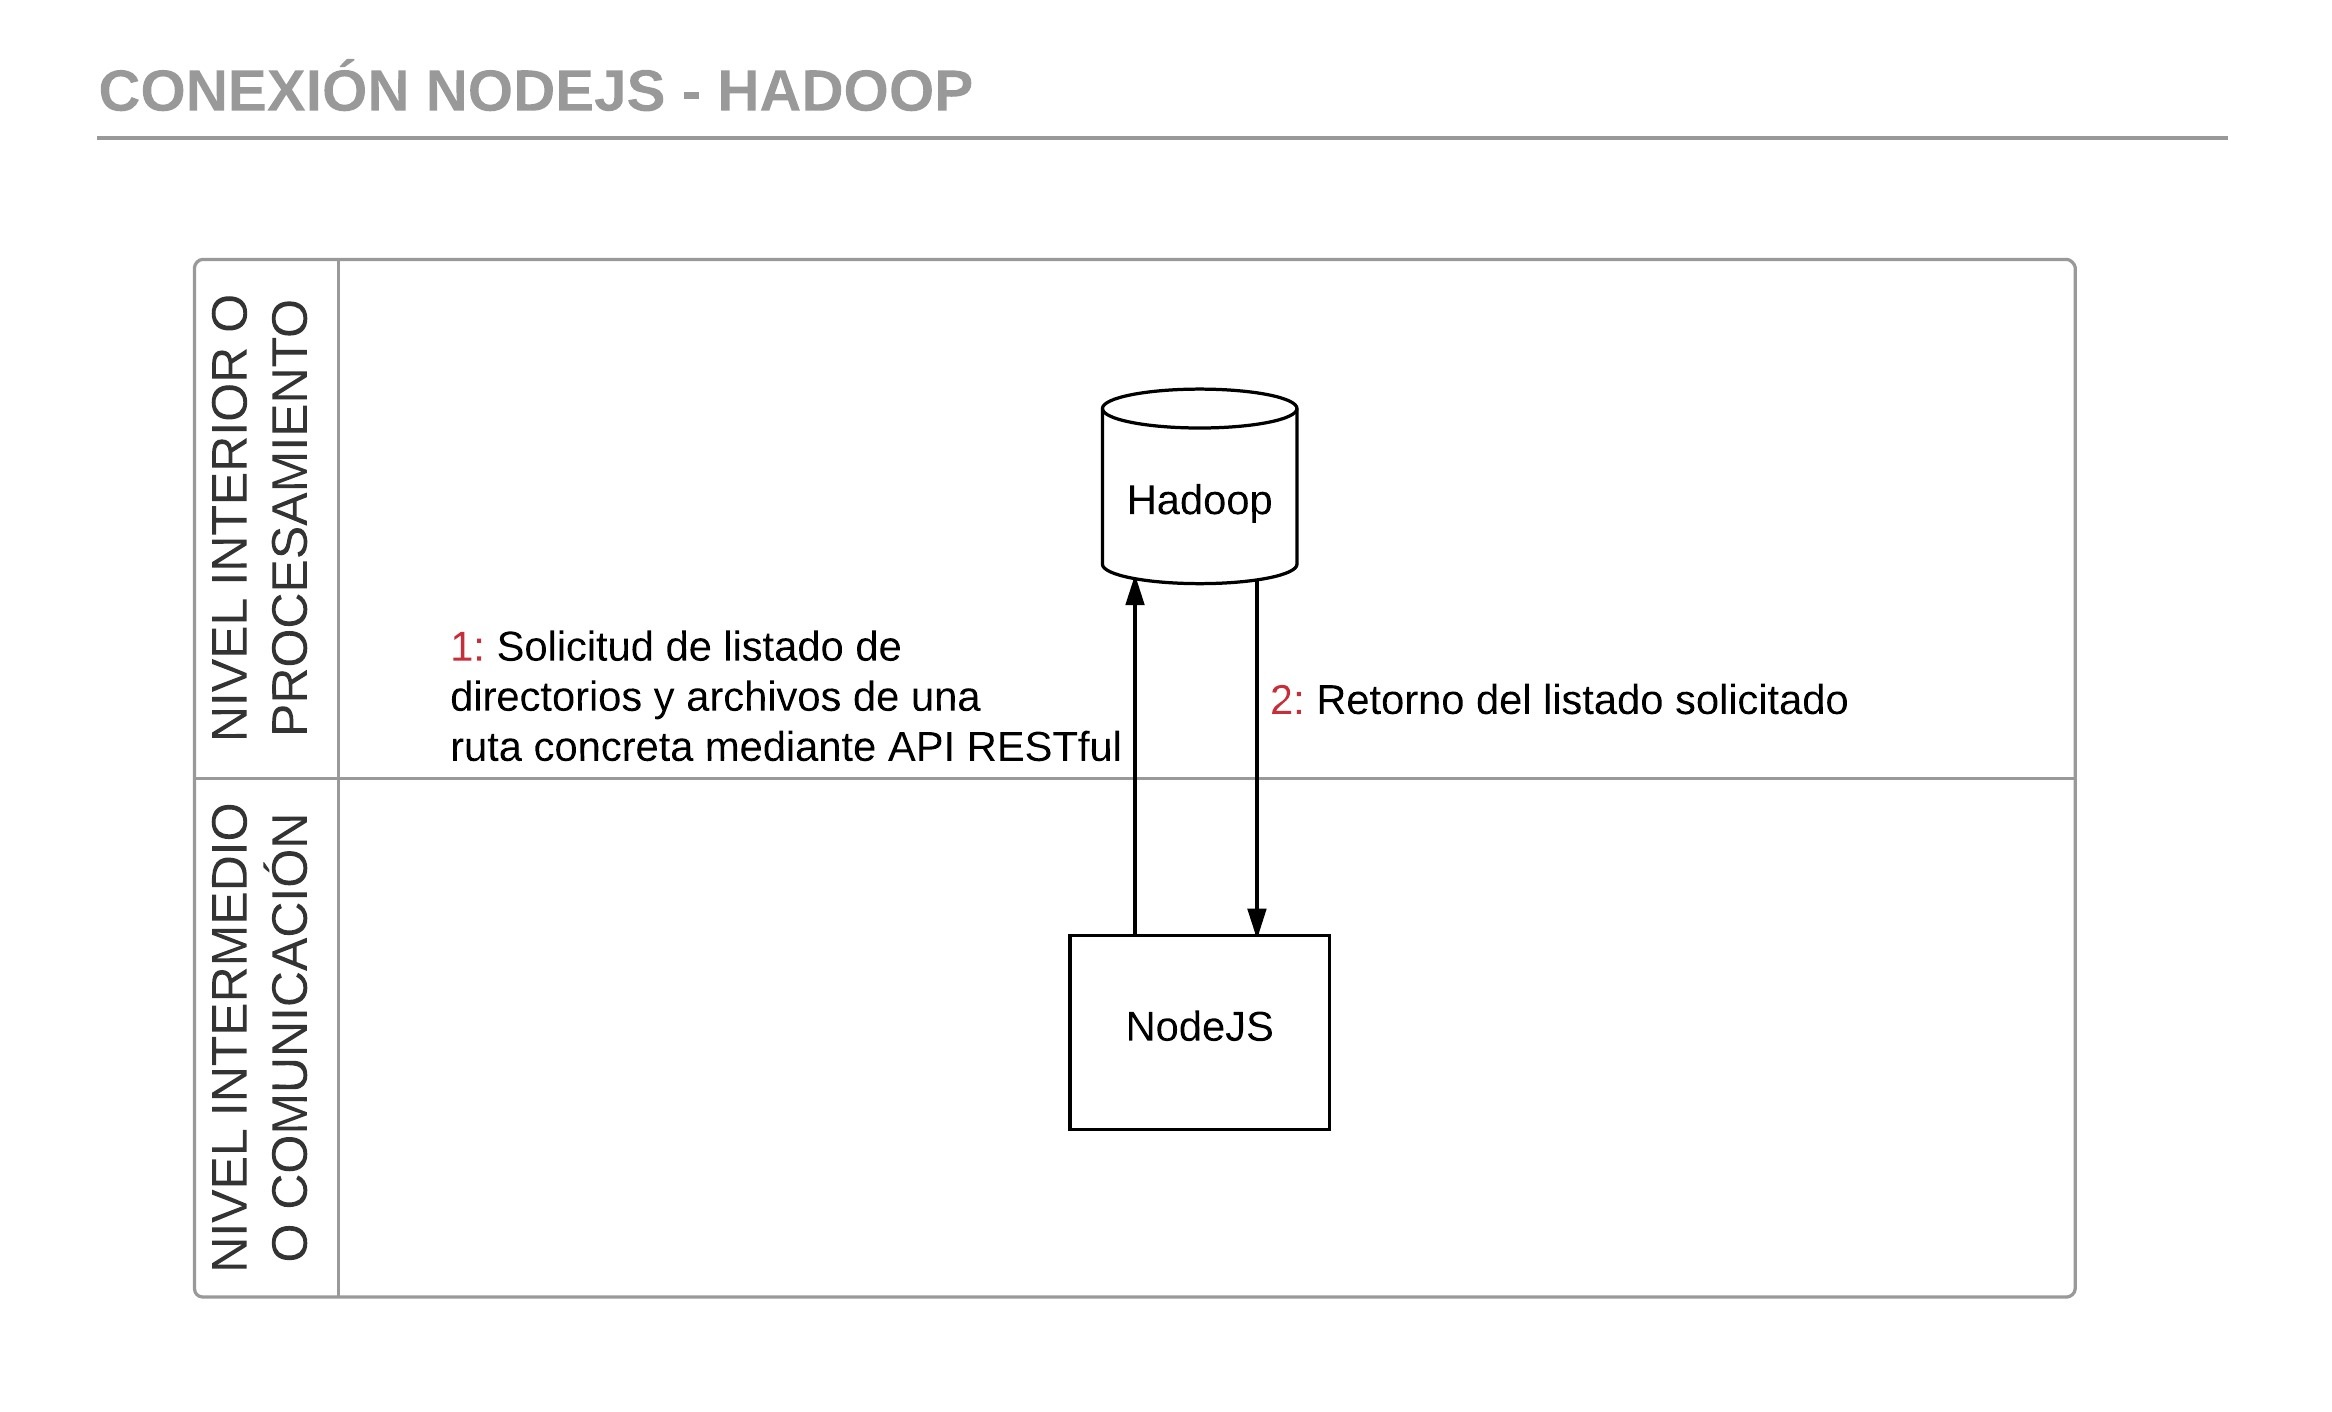
\includegraphics[width=1\linewidth]{imagenes/Conexion_NodeJS_Hadoop}
	\caption{Representación gráfica de la conexión NodeJS - Hadoop}
	\label{fig:conexionnodejshadoop}
\end{figure}


\subsection{NodeJS - Spark}

Existen varias formas de llamar a Spark desde NodeJS. Se puede lanzar un ejecutable a partir de la API RESTful que provee Spark, o lanzar el mismo ejecutable como si se lanzara desde un terminal, a través del comando ‘spark-submit’. Esta segunda opción ha sido la elegida, aunque se ha dejado como un desarrollo futuro la primera, ya que proporciona más información acerca de la ejecución de los códigos creados en Scala. 

\begin{figure}
	\centering
	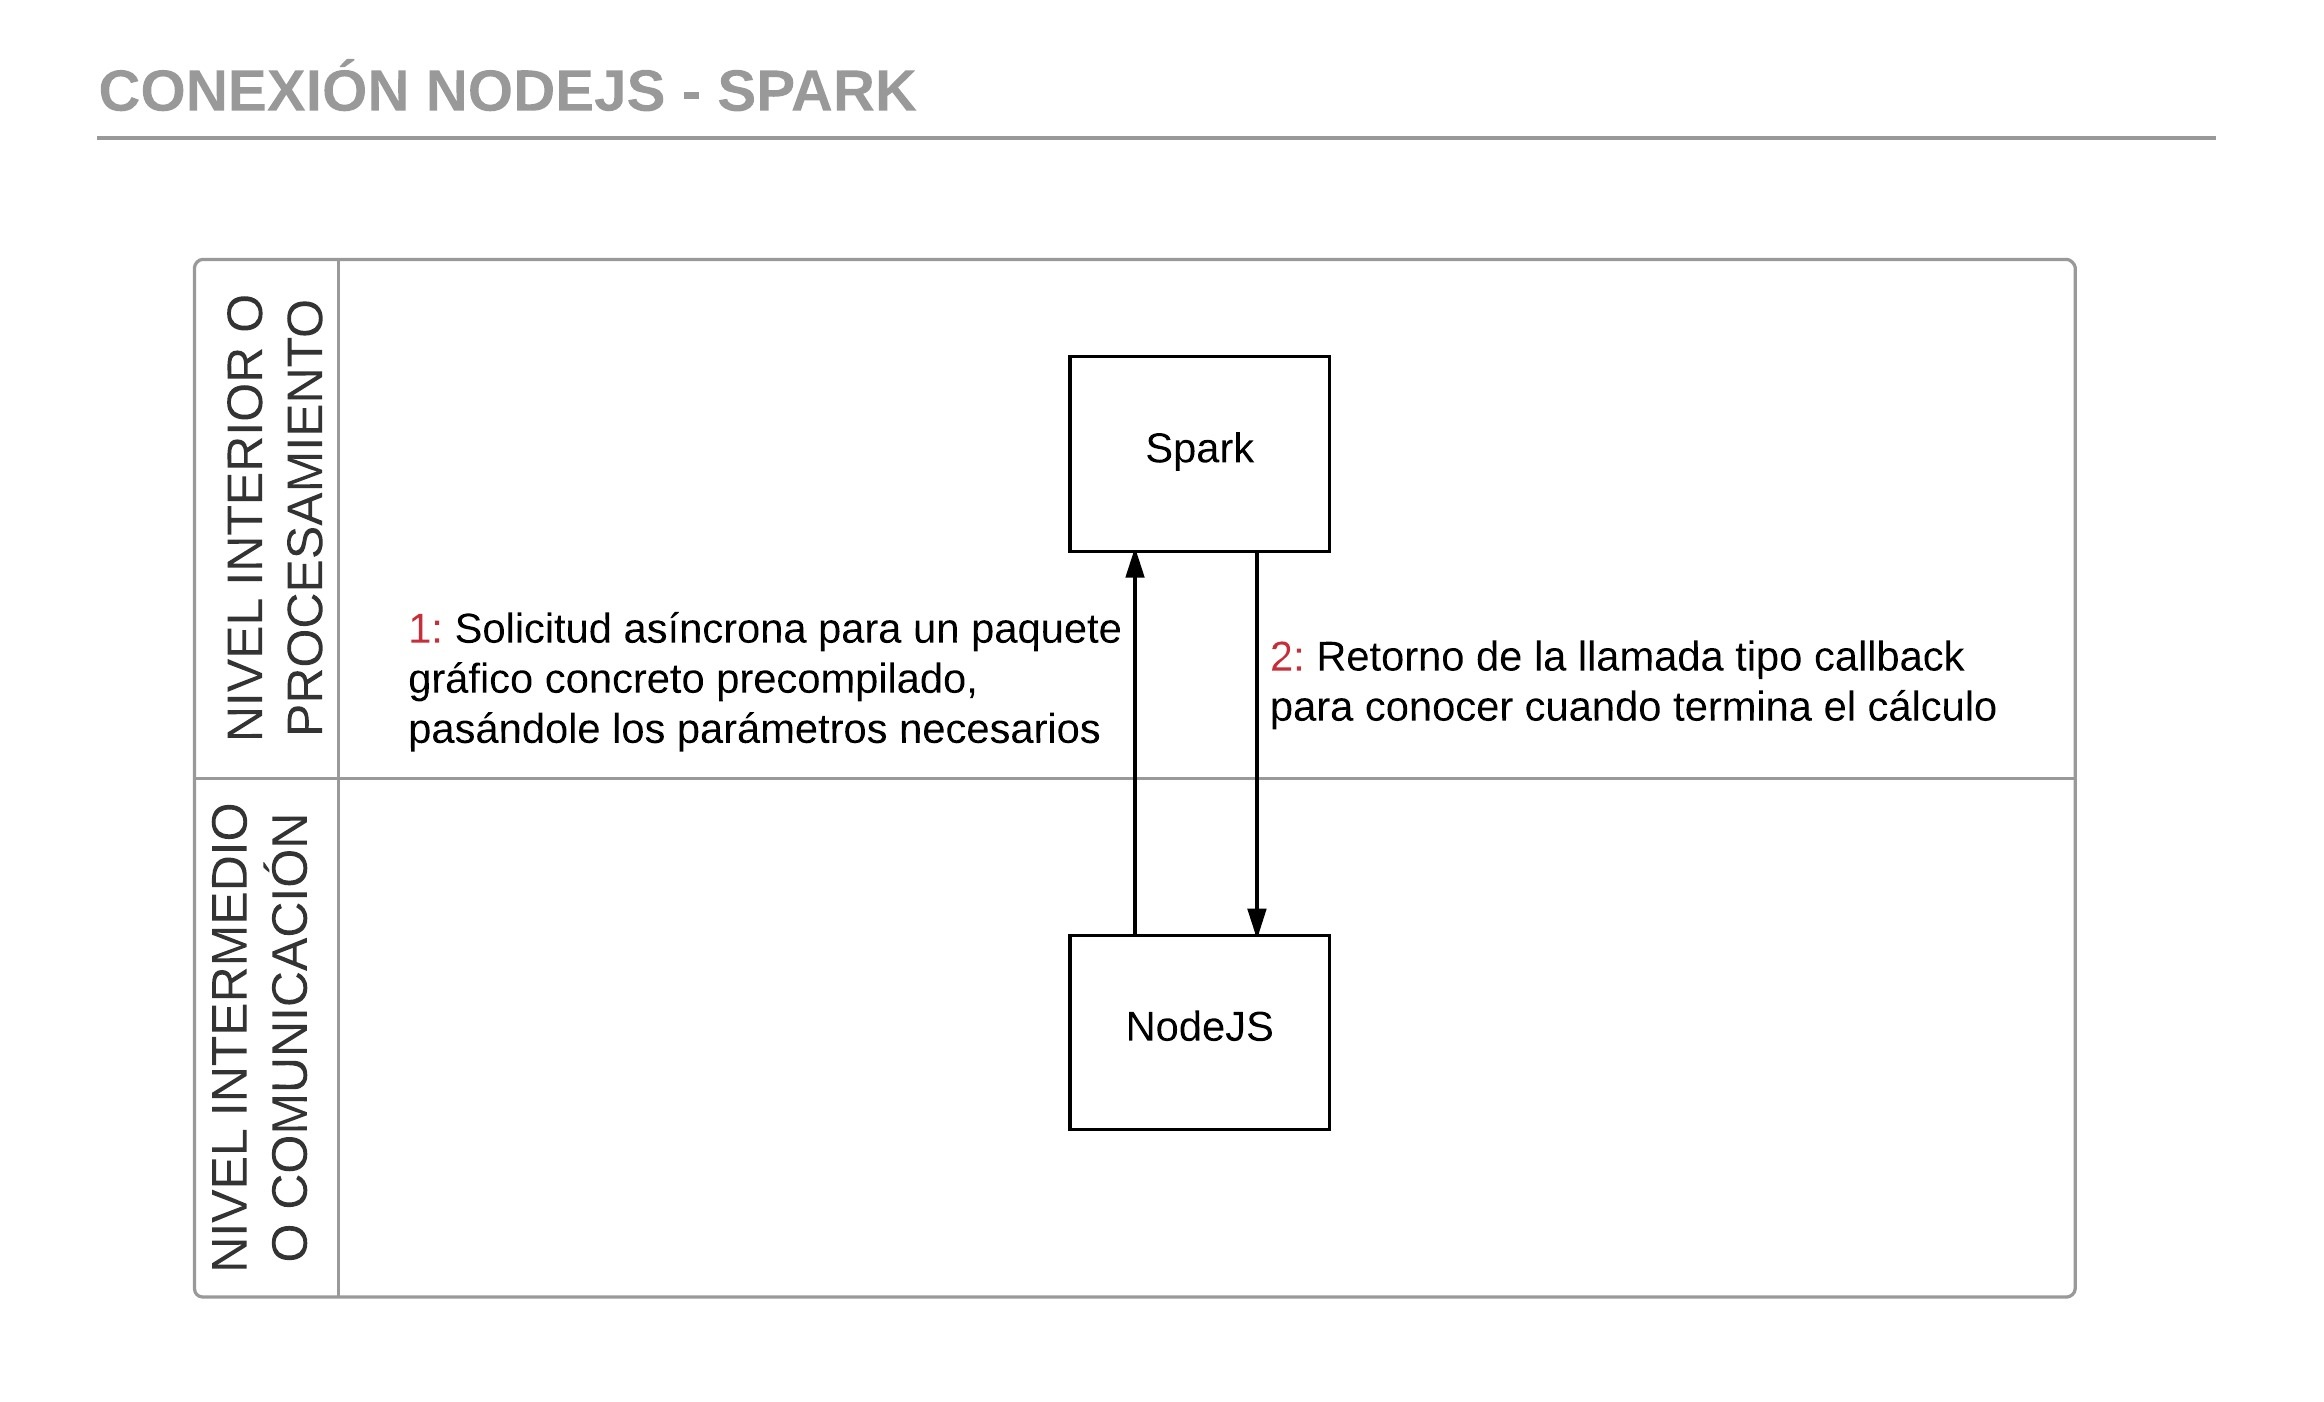
\includegraphics[width=1\linewidth]{imagenes/Conexion_NodeJS_Spark}
	\caption{Representación gráfica de la conexión NodeJS - Spark}
	\label{fig:conexionnodejsspark}
\end{figure}

Teniendo en cuenta esto, es necesario utilizar una librería diseñada para NodeJS llamada ‘node-cmd’ \cite{NodeCmd}, que permite ejecutar comandos como si de un terminal Linux se tratase. Se puede instalar desde el gestor NPM. Además, una de las grandes ventajas es que se puede ejecutar líneas de comandos de manera asíncrona y obtener la salida del mismo en formato String, para almacenarla en una variable si se necesitase. Tiene implementadas dos funciones, ‘run’ que ejecuta el comando y listo, o la función ‘get’, que además se puede indicar una función de tipo ‘callback’ para realizar alguna acción cuando termine la ejecución. En el sistema se ha utilizado la segunda, ya que proporciona más información para seguir trabajando después de la ejecución. 

Cuando se solicite un nuevo gráfico a través de la interfaz web, NodeJS recogerá la información y la pasará al comando ‘spark-submit’ junto con otros datos como la dirección del archivo en el HDFS o la dirección de MongoDB con el nombre de la base de datos y la colección para guardar el resultado. Se puede apreciar el flujo de llamadas en la figura \ref{fig:conexionnodejsspark}

\subsection{NodeJS - MongoDB}

Como ocurre con la conexión con Spark, NodeJS tampoco contiene funcionalidad para conectar con una base de datos en MongoDB. \textbf{Mongoose} \cite{MongooseInicial} es la librería que implementa las herramientas necesarias para lograr este objetivo. Trae consigo mucha funcionalidad para gestionar las bases de datos y las colecciones del sistema MongoDB que esté instalado en el ordenador o cluster. Haciendo una conexión muy sencilla con la función ‘createConnection’, indicándole solamente la URL donde se encuentra la base de datos y la colección, entonces se podrá obtener los documentos en formato JSON que se encuentran alojados en la misma, teniendo la posibilidad de realizar filtros o selecciones concretas sobre los datos. Con esta función se pueden realizar varios accesos de manera concurrente a la base de datos, gestionando ella misma la exclusión mutua. En la figura \ref{fig:conexionnodejsmongodb} se puede ver la conexión entre las herramientas en distintos niveles.

\begin{figure}
	\centering
	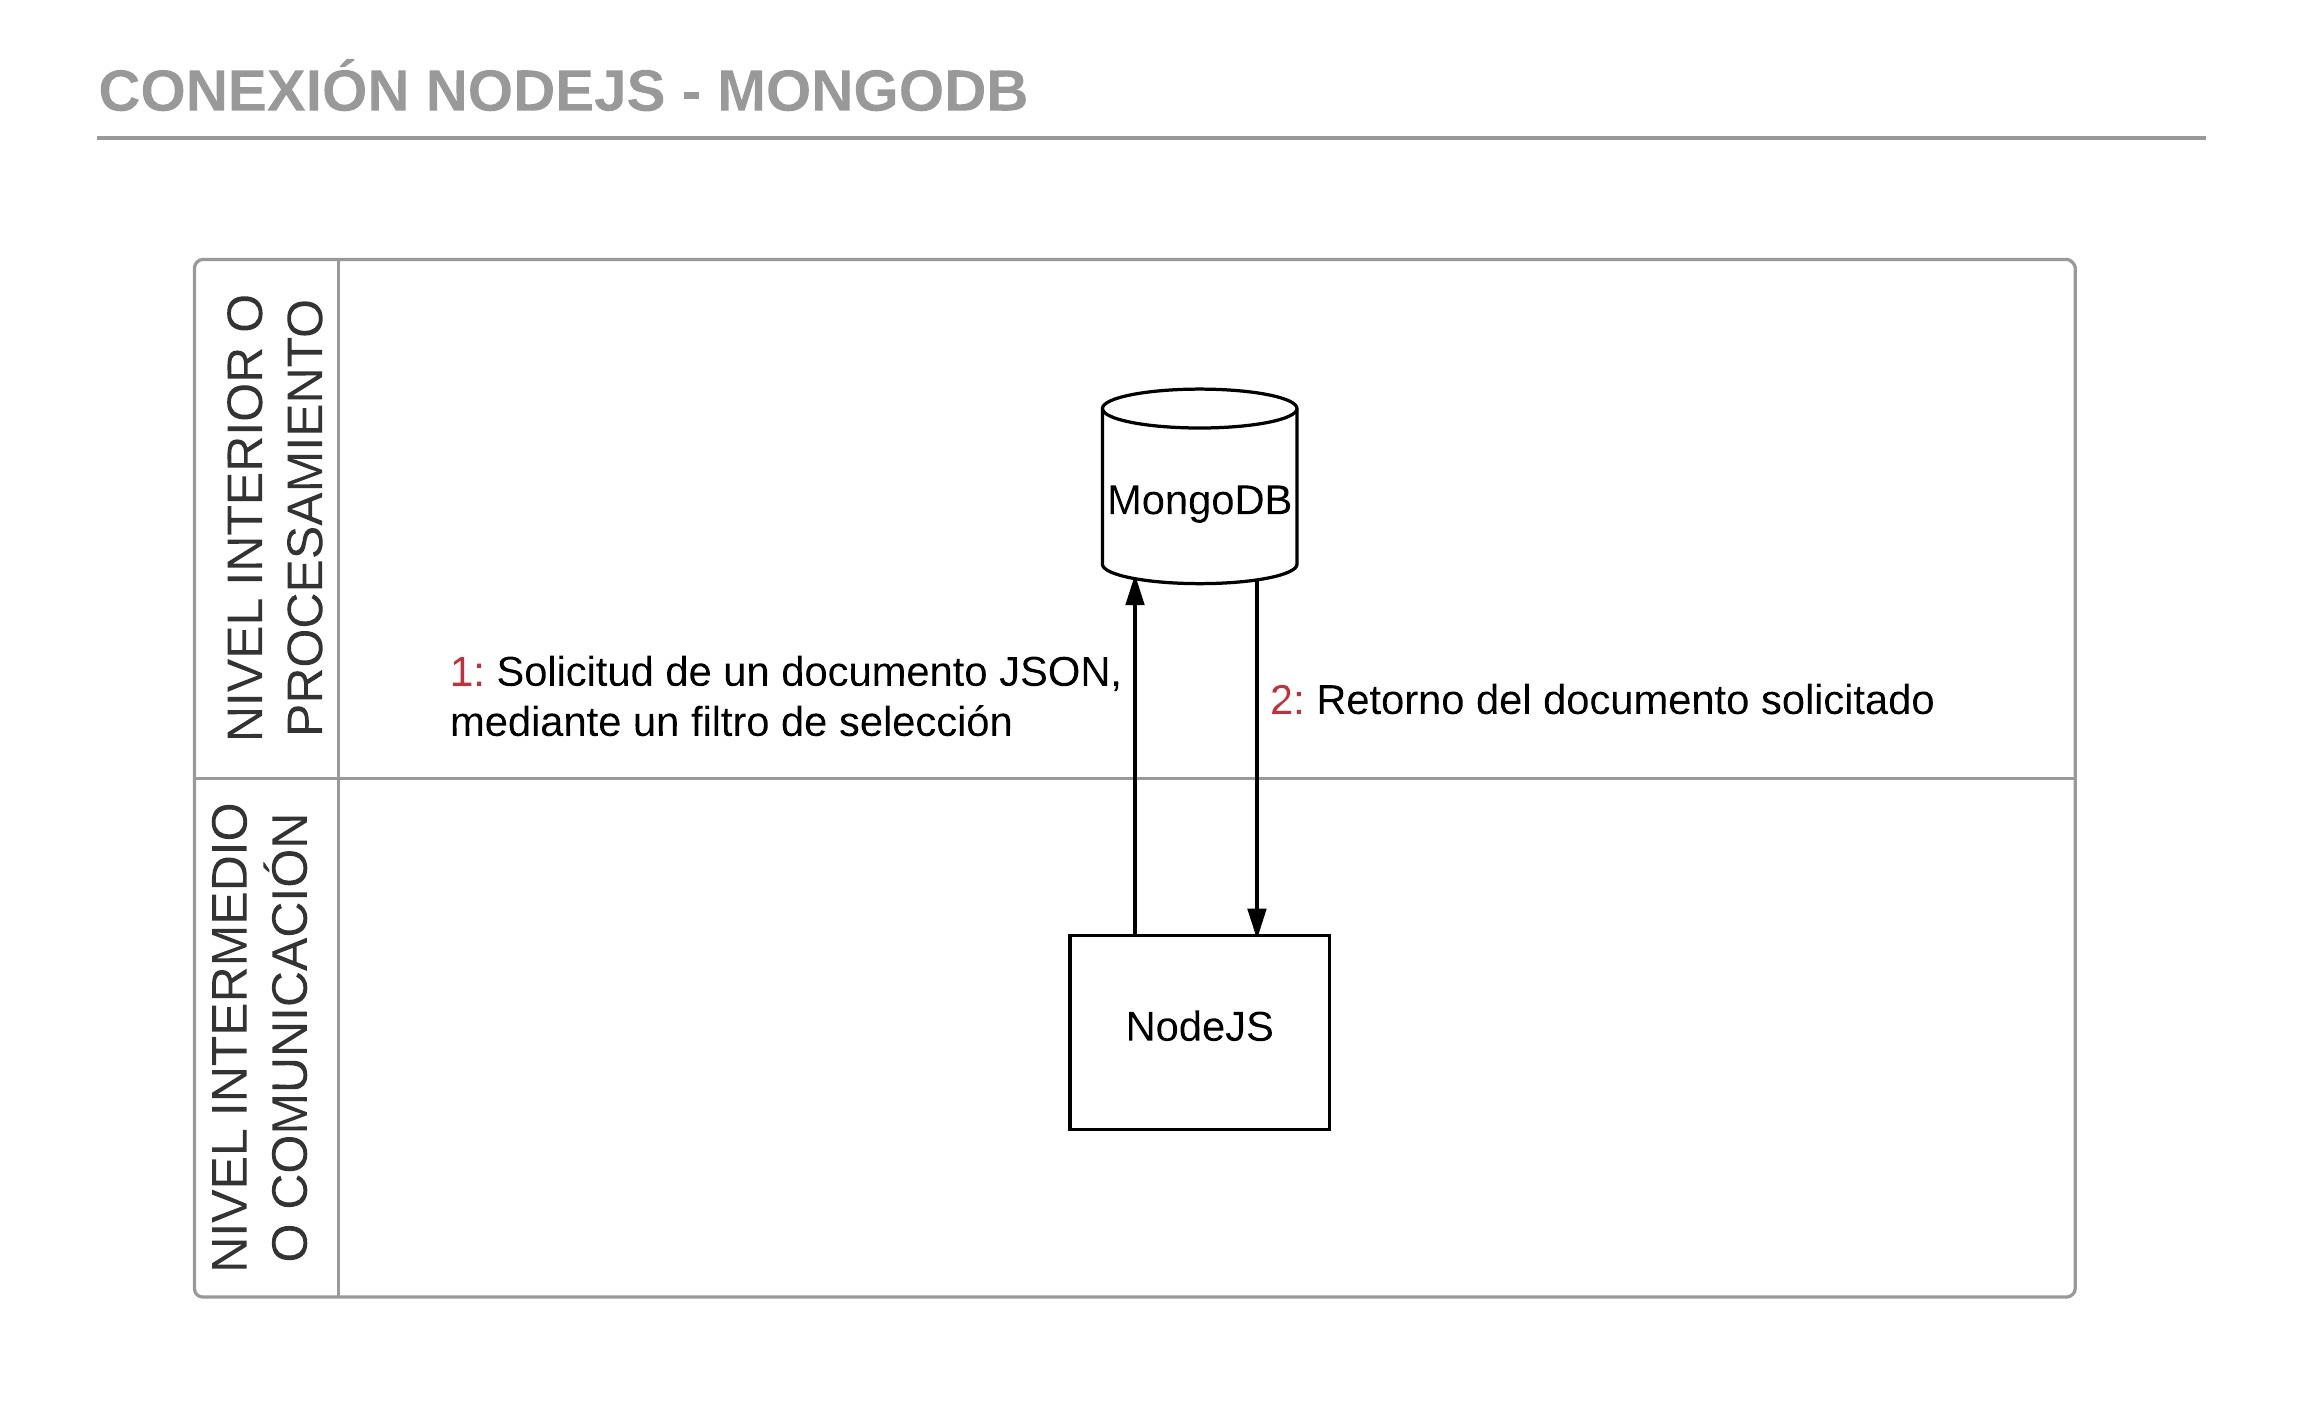
\includegraphics[width=1\linewidth]{imagenes/Conexion_NodeJS_MongoDB}
	\caption{Representación gráfica de la conexión NodeJS - MongoDB}
	\label{fig:conexionnodejsmongodb}
\end{figure}

En el sistema, se utiliza para dos cosas. La primera es para insertar y modificar los documentos que mantienen el estado de una ejecución, dentro de una colección habilitada para ello. Ahí se almacena el identificador de la ejecución, el estado en el que se encuentra y las fechas de inicio y fin. La segunda es para buscar el resultado que ha dejado Spark en la colección de la base de datos específica, filtrando los datos por el identificador que se generó previamente.

\subsection{NodeJS - D3JS}

D3JS es una librería muy potente que permite generar desde sencillos gráficos hasta de los más complejos, dándole incluso dinamismo. En NodeJS se puede integrar a través del gestor de paquetes NPM, para poder acceder a la amplia gama de funciones para generar los infogramas. La propia librería provee una galería de gráficos de ejemplo \cite{D3JSGallery} para ayudar a implementar cualquiera. Al ser totalmente abierta, el desarrollador es libre de modificar cualquiera de estos ejemplos a sus propias necesidades, o incluso diseñar uno desde cero.

Dentro de esta galería, se han utilizado uno o varios ejemplos para la creación del listado de gráficos disponibles en la API, adaptándolos a los datos resultados. Ya que no es viable generar un gráfico con todos los datos que puede contener dentro del concepto de ‘Big Data’, por eso son necesarias las técnicas de reducción y agrupación de las que se encarga Spark, teniendo en cuenta que los resultados que se dibujen en la gráfica sean representativos de lo que ocurre con los datos. 

Cabe destacar que forma parte de la propia experiencia del usuario de la API, seleccionar el gráfico adecuado para los datos seleccionados

\subsection{Interfaz web - NodeJS}

La conexión de NodeJS con la interfaz web, sigue una estructura de cliente-servidor. Es el propio usuario el que solicita información a través de la web al servidor, el cual debe retornar lo solicitado dentro de un tiempo razonable. NodeJS implementa una conexión nativa con las aplicaciones web, permitiendo la comunicación entre ambas partes, como se puede ver en la figura \ref{fig:conexioninterfaznodejs}.

\begin{figure}
	\centering
	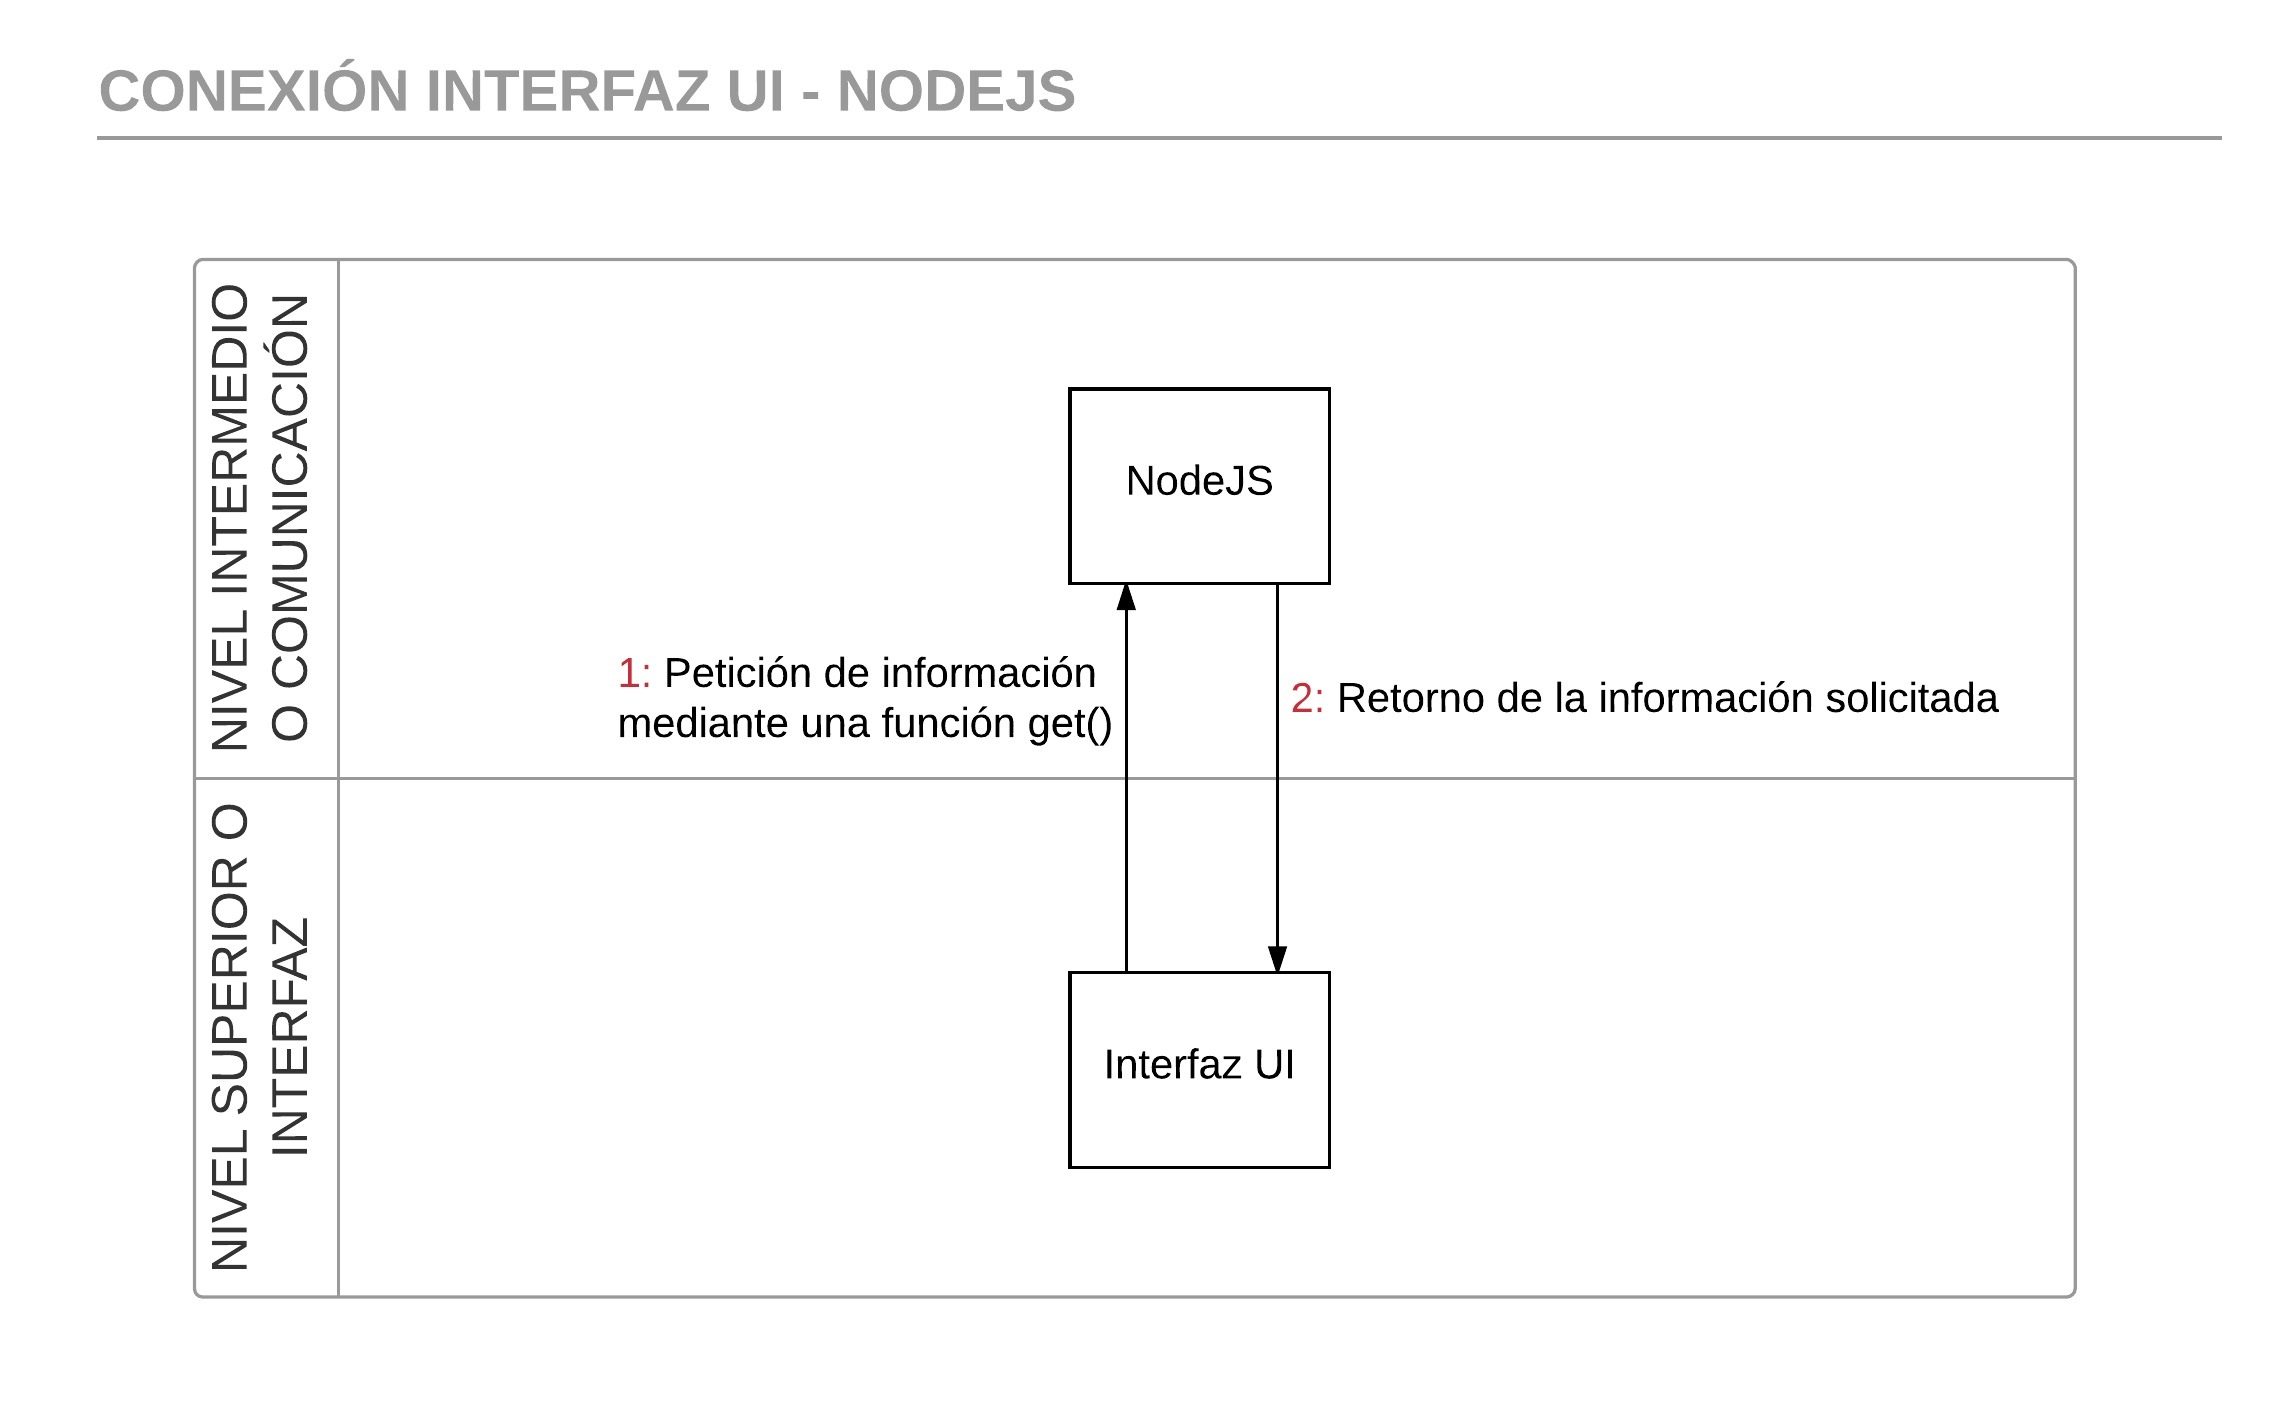
\includegraphics[width=1\linewidth]{imagenes/Conexion_Interfaz_NodeJS}
	\caption{Representación gráfica de la conexión Interfaz web - NodeJS}
	\label{fig:conexioninterfaznodejs}
\end{figure}

Además, NodeJS trae implementado un gestor de plantillas de tipo JADE (o PUG renombrado en las últimas versiones) \cite{PugInicial}. Pug es un motor de plantillas, diseñado para simplificar la escritura de código HTML, que está integrado en NodeJS. Con Pug se resume la cantidad de código que es necesario escribir para el diseño de una página HTML, siguiendo una estructura muy sencilla. NodeJS se encarga de traducir las plantillas escritas en Pug a código HTML, para que el navegador web pueda ejecutarlo. Cabe destacar que cuando se comenzó con este proyecto, todavía era Jade, dejando como tarea a desarrollar la actualización del contenido escrito en esta plantilla.

\section{Flujo de procesamiento}

En este apartado se va a explicar cómo funciona internamente el sistema cuando se solicita alguna de las funcionalidades disponibles desde la interfaz web. Lo primero es listar las funciones que se pueden realizar y explicar cada una por separado. 

\subsection{Mostrar el listado de archivos y directorios en el HDFS}

Desde la interfaz, el usuario solicita, o el propio sistema automáticamente al iniciar la API, a NodeJS listar el contenido de un directorio específico dentro del HDFS. En el caso del inicio del sistema, se solicita el directorio raíz. Después NodeJS es el encargado de pedir y recuperar esta información a Hadoop, para a continuación, devolverla a la interfaz, que será la encargada de darle el formato correcto. En la figura \ref{fig:listararchivosdelhdfs} se puede apreciar gráficamente el flujo de llamadas entre las herramientas.

Cabe destacar que el sistema solo trata actualmente con ficheros de tipo CSV y que no estén vacíos. Ampliar el número de tipos de ficheros permitidos es una de las principales mejoras de este sistema.

\begin{figure}
	\centering
	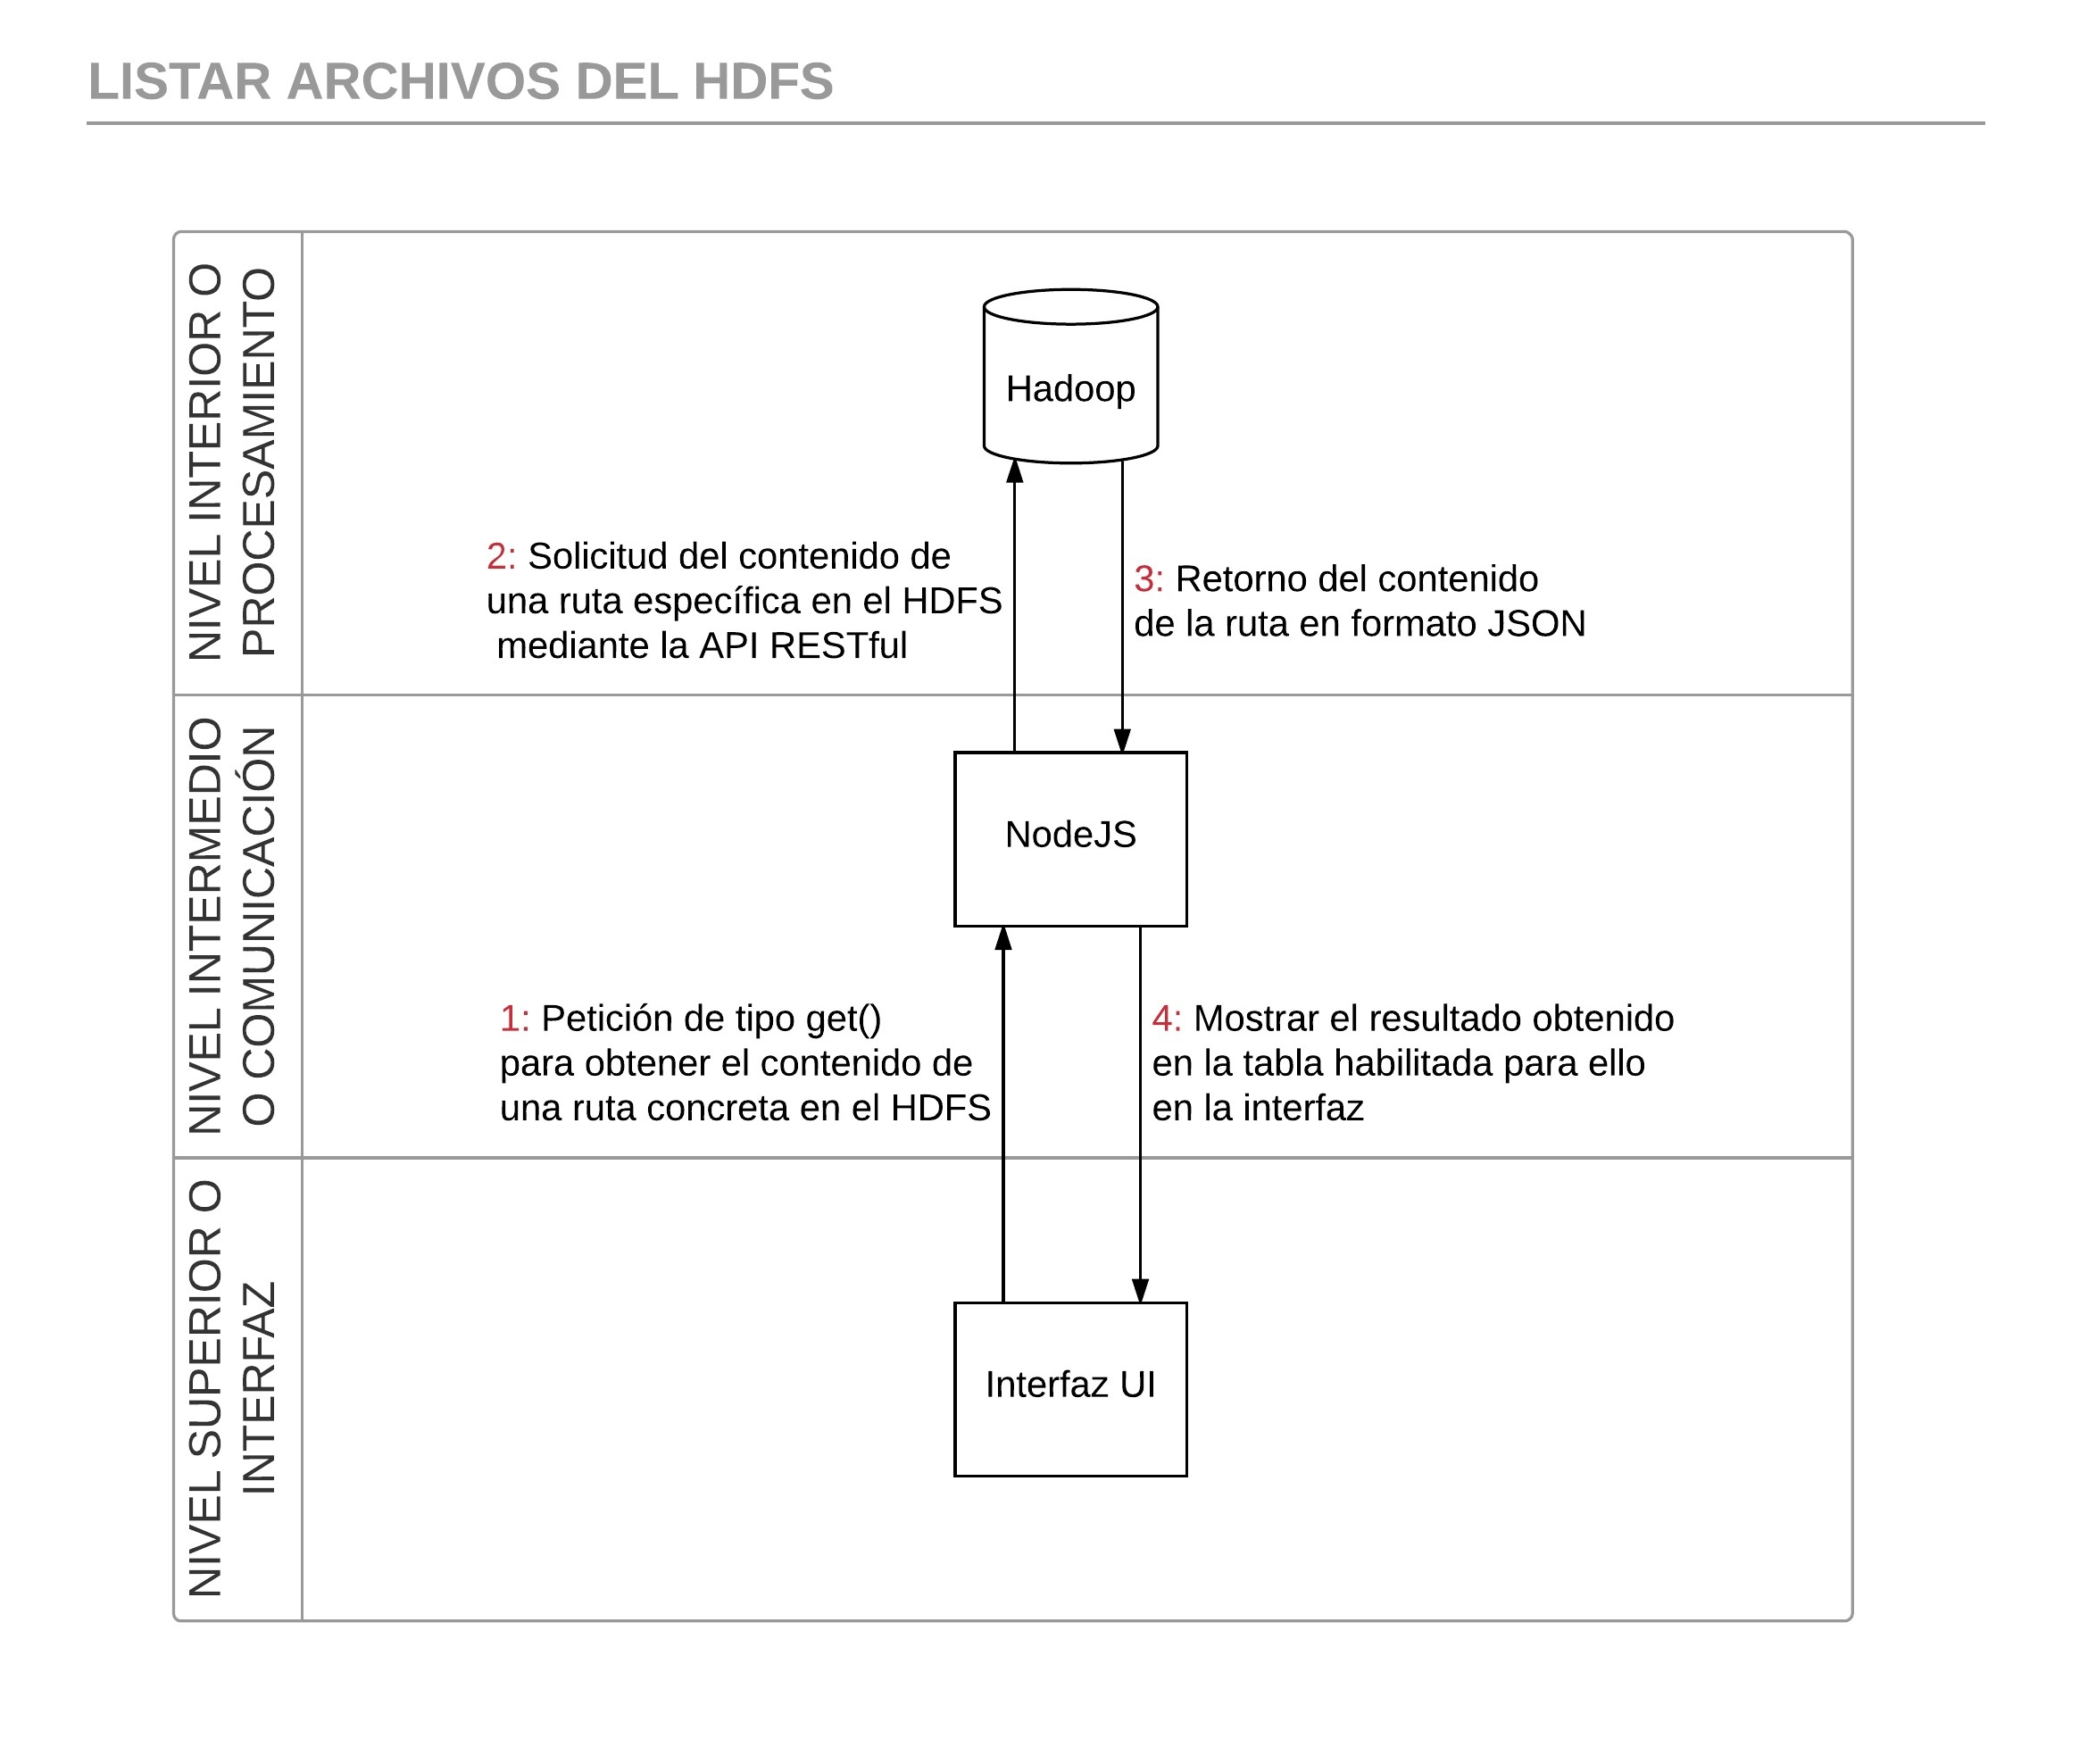
\includegraphics[width=1\linewidth]{imagenes/Listar_archivos_del_HDFS}
	\caption{Flujo de llamadas para listar el contenido del HDFS}
	\label{fig:listararchivosdelhdfs}
\end{figure}

\subsection{Ejecución de un proceso seleccionado}

Ya se trate de mostrar el resumen de un fichero seleccionado, solicitar un gráfico bajo unos parámetros concretos o simplemente mostrar los datos de dicho gráfico, el proceso que realiza el sistema internamente es el mismo. 

El primer paso es la solicitud de mostrar esa información por parte del usuario. Para ello, la interfaz web recoge los parámetros que necesita para ejecutar la función correspondiente. Si es para mostrar la información resumen del contenido de un fichero, basta con enviarle a NodeJS que fichero es y en que ruta está almacenado. En el caso que se quiera un gráfico o los datos resultados directamente, habrá que añadir todos los parámetros indicados en el formulario de la interfaz habilitado para cada uno de los infogramas disponibles. 

A continuación, NodeJS genera un identificador del proceso a partir de la ruta del fichero seleccionado, el tamaño del mismo, el gráfico que se desea generar y sus parámetros. Con el identificador creado, antes de realizar ninguna acción más, comprueba que el resultado del proceso no se encuentre ya en la colección, o esté calculándose paralelamente a este. En cuyo caso, el sistema se esperaría a que estuviese terminado para recuperar la información, evitando guardar resultados duplicados. Cuando terminase, devolverá el resultado a la interfaz para visualizarlo. Esta comprobación se explica gráficamente en la figura \ref{fig:procesoyaejecutadopreviamente}.

\begin{figure}
	\centering
	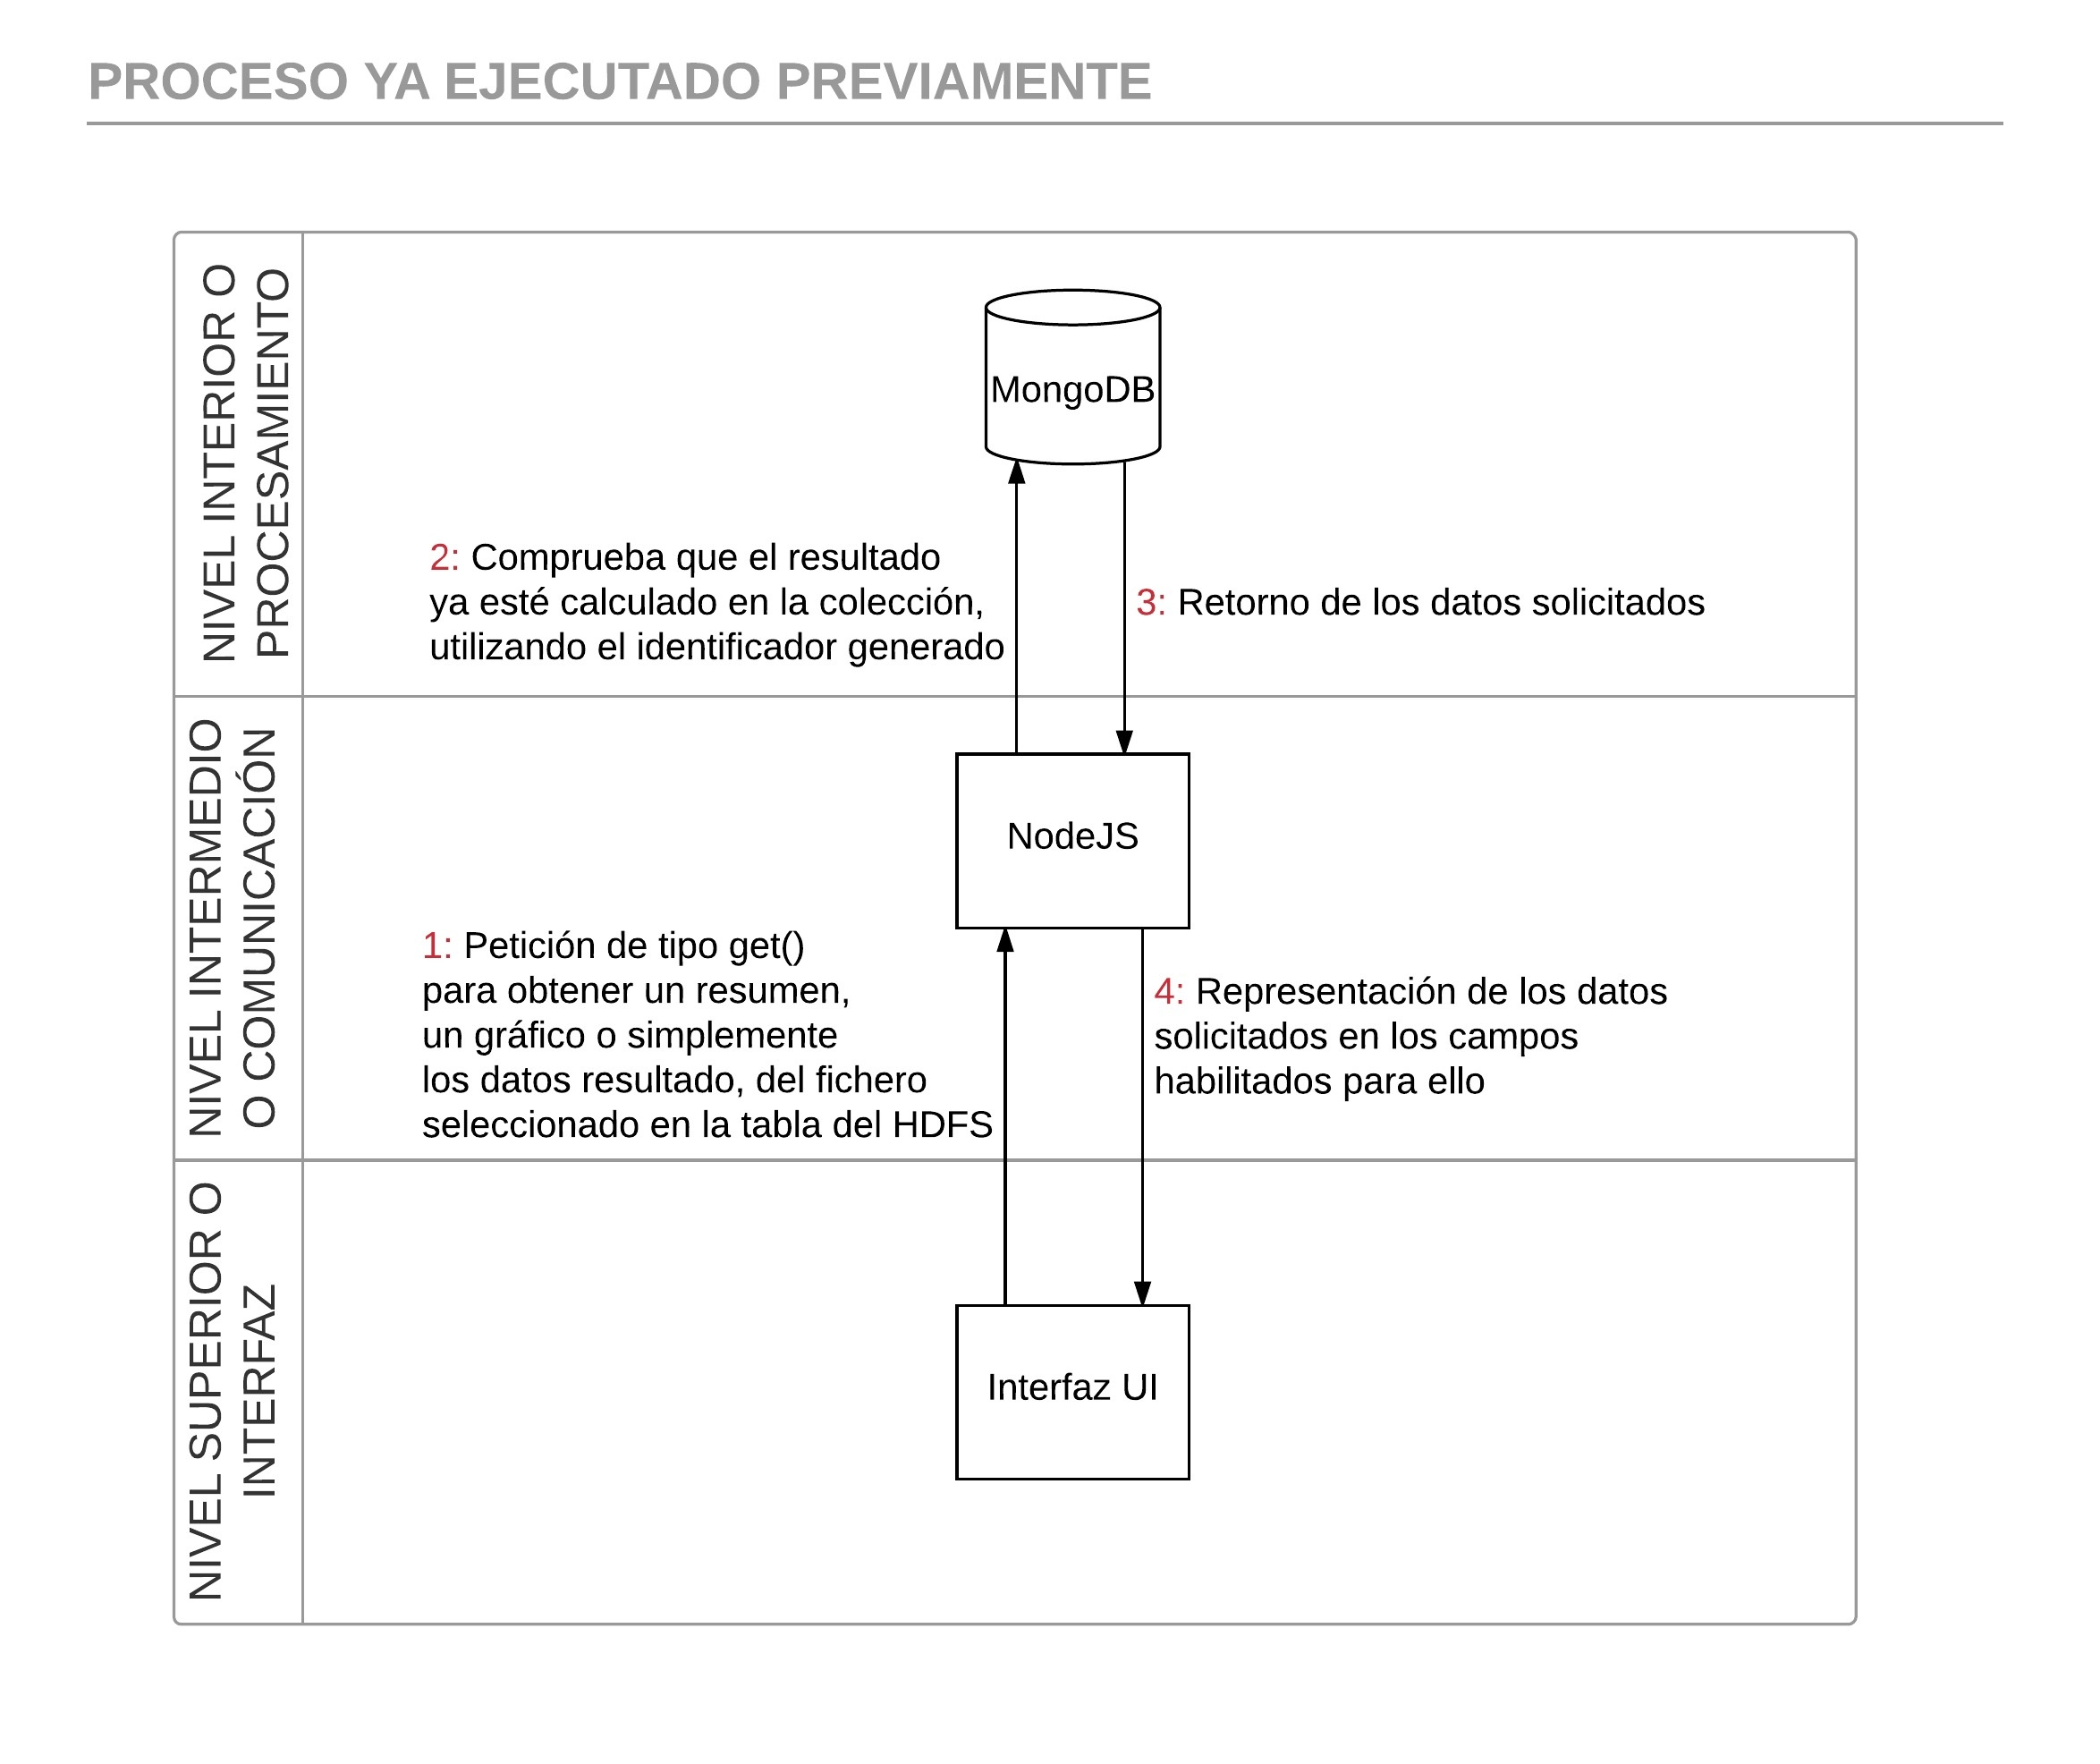
\includegraphics[width=1\linewidth]{imagenes/Proceso_ya_ejecutado_previamente}
	\caption{Ejecución de un proceso ya generado anteriormente}
	\label{fig:procesoyaejecutadopreviamente}
\end{figure}

Si no estuviera el resultado, tal y como se indica en la figura \ref{fig:ejecuciondeunproceso}, el siguiente paso sería generar un documento JSON con la información del estado actual del proceso y guardarlo en una colección habilitada para ello en MongoDB.

\begin{figure}
	\centering
	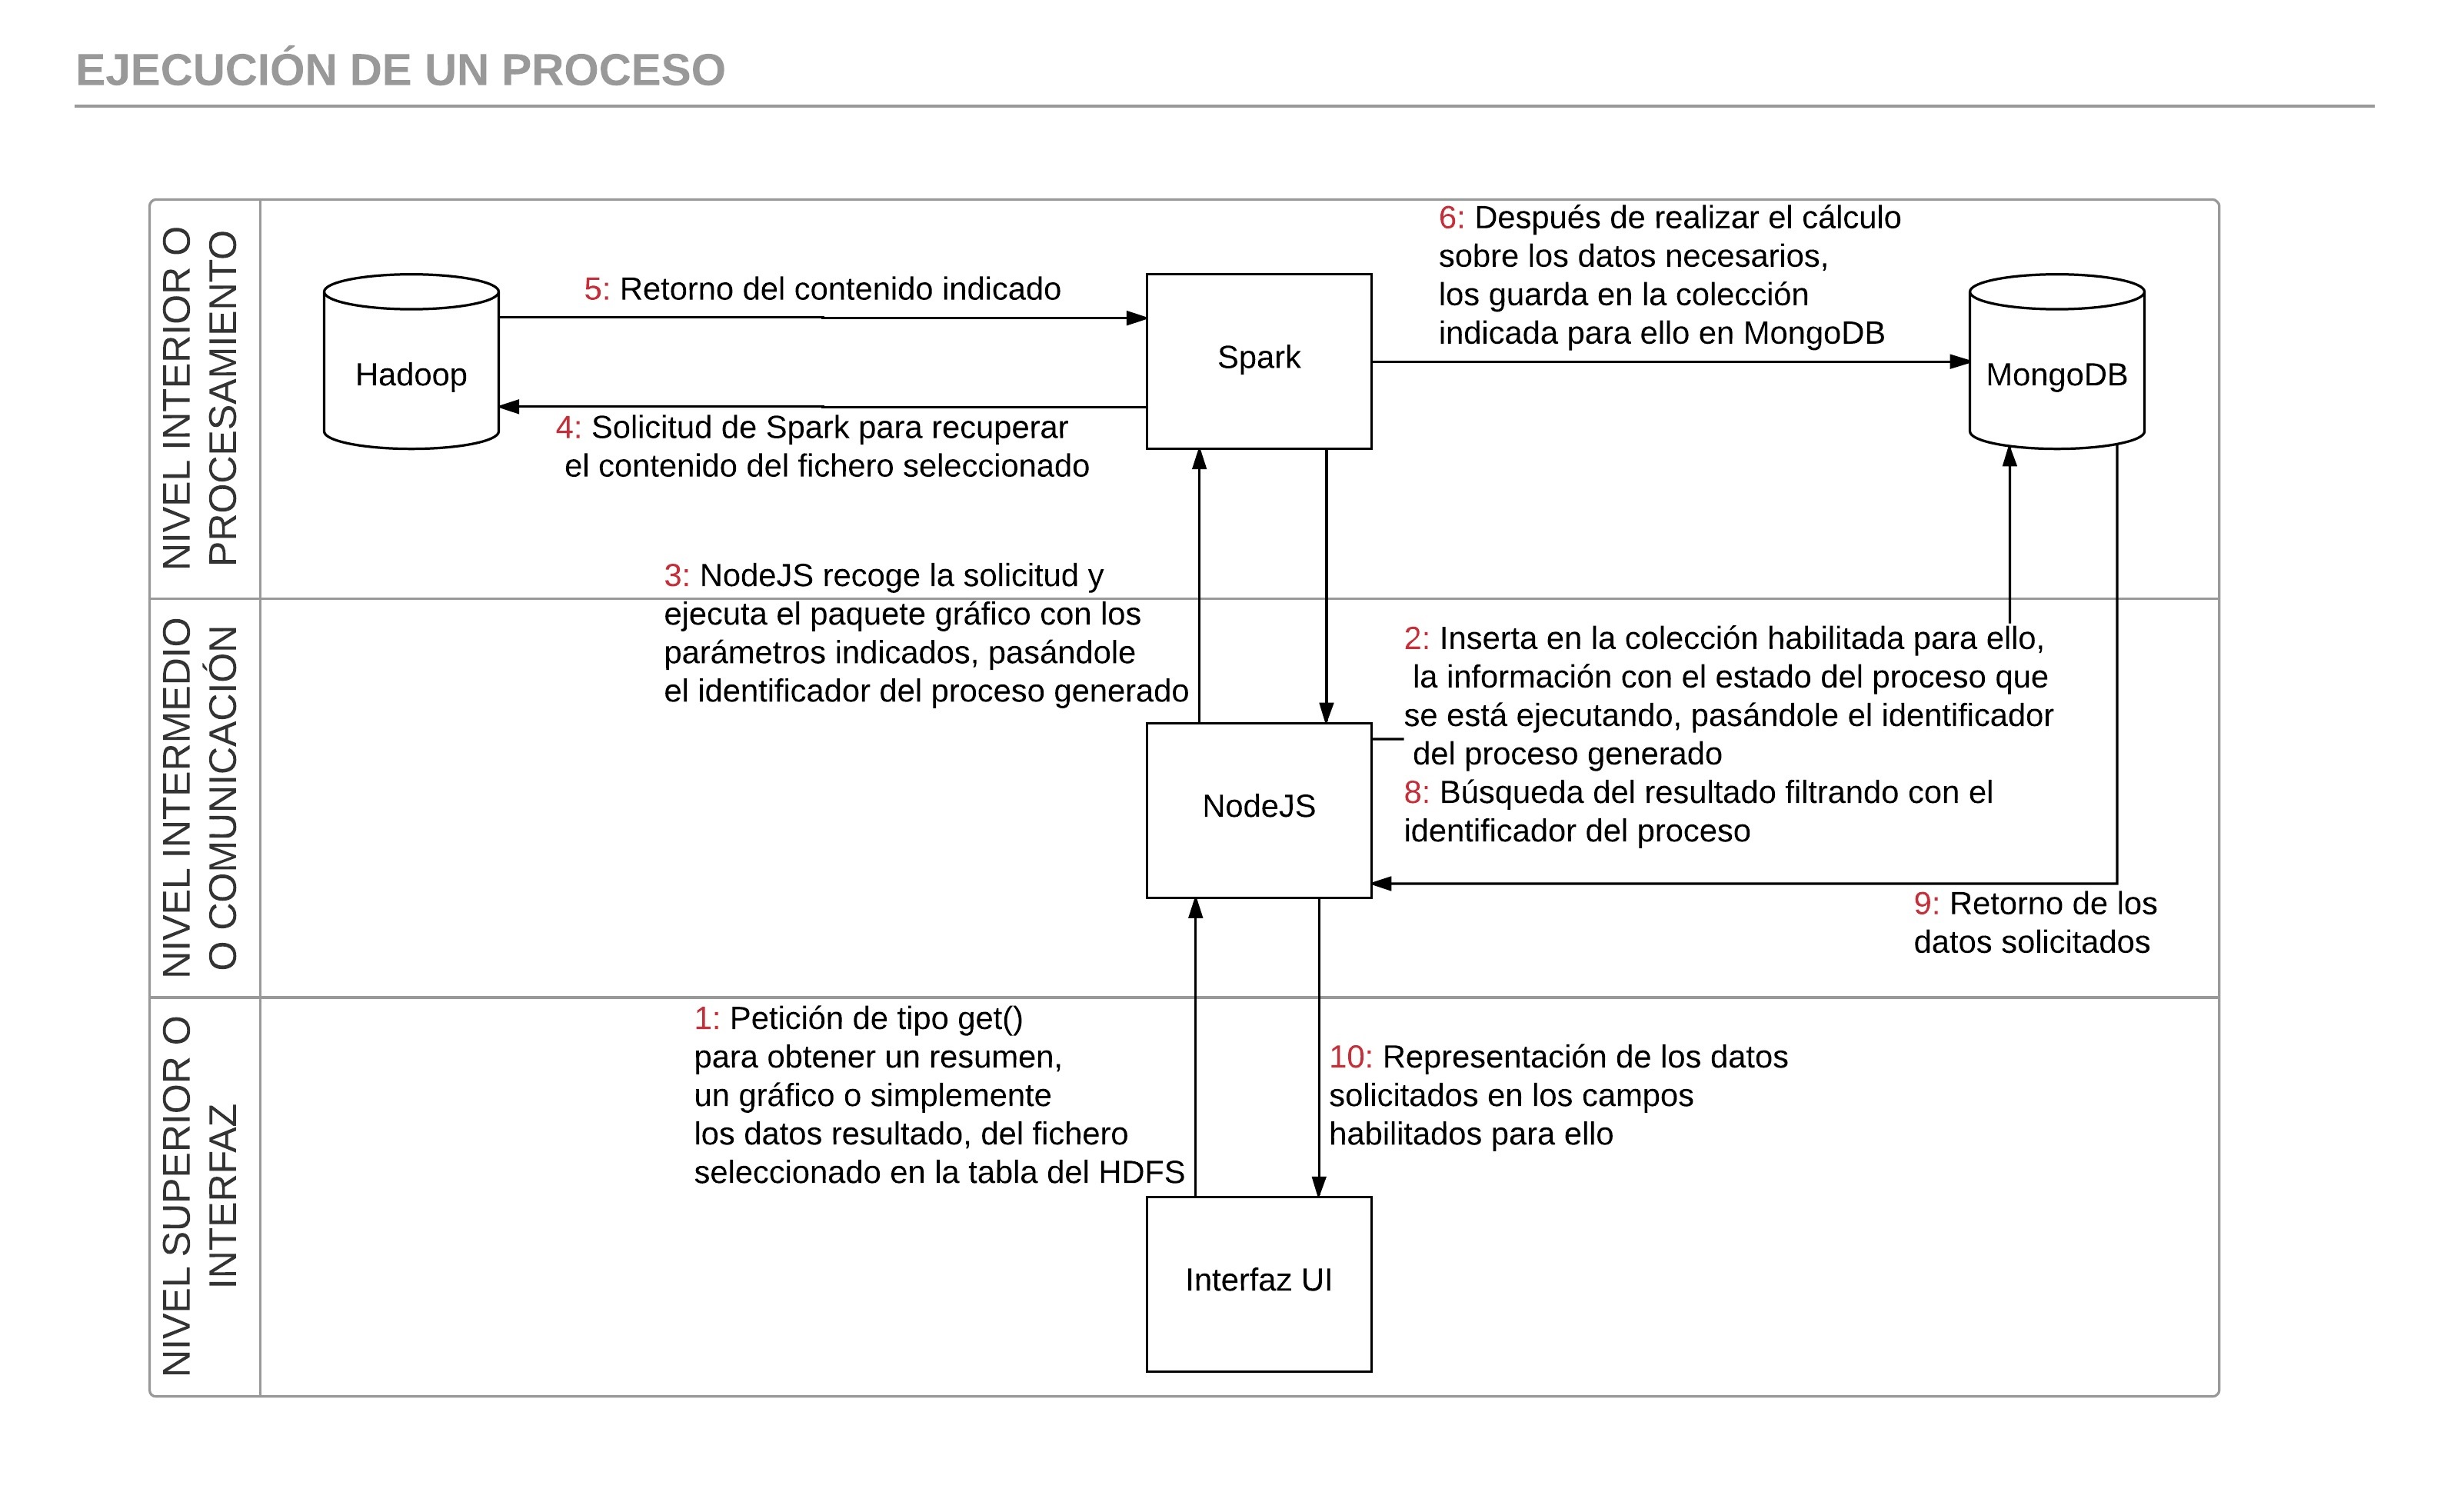
\includegraphics[width=1\linewidth]{imagenes/Ejecucion_de_un_proceso}
	\caption{Ejecución de un proceso solicitado}
	\label{fig:ejecuciondeunproceso}
\end{figure}

Ejecutar el paquete gráfico es el siguiente paso, enviándole la información de los parámetros indicada anteriormente, junto con el identificador. 

Dentro del paquete en Spark, como ya se explicó, primero se recupera el archivo del HDFS. En el caso del paquete ‘summary’, basta con obtener algunos metadatos del fichero, como la cantidad de columnas que contiene, los nombres de las mismas o el número de registros, entre otros. Si se está ejecutando un proceso gráfico, entonces el propio paquete contendrá el esquema de agrupación y las técnicas de reducción de datos que debe ejecutar para obtener el resultado correcto. Finalizado este cálculo, Spark guarda en la colección de MongoDB, el resultado junto al identificador del proceso. 

Cuanto termina de ejecutarse la librería, NodeJS busca el resultado en MongoDB, utilizando como filtro el identificador. Por último, regresará la información a la interfaz para visualizarla en los campos indicados para ello.

\section{Instalación del sistema de visualización y BigData}

Como ya se han explicado con anterioridad, los componentes necesarios para la utilización de la API son:
\begin{itemize}
	\item Spark (2.0)
	\item Hadoop (2.6)
	\item Scala (2.11)
	\item Java JDK (1.7 o superior)
	\item MongoDB (3.2)
	\item NodeJS (6.9)
	\item Sbt (0.13)
\end{itemize}

Cabe destacar que es posible que se pueda instalar la API con otras versiones de alguna de las herramientas listadas anteriormente, pero no se garantiza la correcta funcionalidad de la misma.

Es posible una instalación básica del sistema de todos estos componentes de manera automática, excepto de Hadoop, mediante el fichero installAll.sh, proporcionado dentro del directorio del proyecto en GitHub, para sistemas CentOS, Fedora, RedHat, etc. Esta instalación está basada en los requisitos mínimos para que el sistema funcione, en un solo nodo para Hadoop y Spark. La instalación de Hadoop es más complicada y por ello se debe realizar manualmente. En sistemas Debian, la instalación debe ser manual. La única diferencia es el cambio en los nombres de algunos de los comando utilizados en sistemas Debian. La instalación básica requiere de al menos 8 GB de RAM y al menos ocupa 4GB de espacio en disco.

\underline{Importante}: Para que el sistema funcione con el firewall activado, es necesario tener abiertos los puertos que solicita cada una de las herramientas como Hadoop, Spark, etc. En caso contrario, se deshabilitara el firewall para poder ejecutar la API sin ese problema. Los siguientes comando lo deshabilitan para Centos 7. (Estos comandos ya están añadidos en el fichero installAll.sh)

\begin{verbatim}
	systemctl disable firewalld
	
	systemctl stop firewalld
\end{verbatim}

También es importante abrir el puerto del ordenador o cluster que se le indique en la configuración de la API.

Para la instalación de Hadoop y Spark sobre un cluster de varios nodos, se ha seguido el siguiente tutorial \cite{InstalacionHadoopSparkNodos} proporcionado por el tutor del proyecto. La instalación de NodeJS y el resto de componentes se realiza de la misma forma que en la versión básica explicada anteriormente. 

\section{Compilación de los paquetes gráficos}

Para que el sistema pueda ejecutar cada uno de los paquetes que calculan los datos resultados necesarios para los gráficos, es necesario tener instaladas las siguientes herramientas como mínimo:
\begin{itemize}
	\item Spark
	\item MongoDB
	\item Hadoop
	\item Scala
\end{itemize}

Lo primero es compilar el paquete. Dentro del proyecto ya vienen compiladas las funciones de cada uno de los gráficos, pero si se realizan cambios sobre el código de alguno de ellos, es necesario volver a compilar. 

Para ello, es necesario situarse dentro del directorio del gráfico (histogram, boxplot, ...) y utilizar el comando "sbt assembly". A continuación, se generará un paquete .jar en ./target/scala-2.11/X-assembly-1.0.jar, donde X será el nombre del gráfico a compilar y dependiendo de la versión de Scala que esté instalada. Este paquete contendrá todas las librerías privativas necesarias para su correcto funcionamiento, indicadas dentro del fichero ‘build.sbt’, en el directorio de cada uno de los gráficos.

Dentro de estos directorios, existe un ejecutable 'launch.sh', donde se puede probar la funcionalidad del mismo paquete, con algunos datos de prueba. En la sección número 6 de este documento, se especifica que parámetros se deben introducir en cada uno de los gráficos. Tener en cuenta que se necesitan datos dentro del HDFS y que el resultado de la ejecución, se guardará en MongoDB, además de ajustar los parámetros de conexión a las condiciones de cada servidor y de cada ejecución.

\section{Uso de la biblioteca}

Durante el desarrollo del sistema, se ha utilizado una herramienta de documentación y testeo sobre NodeJS llamada \textbf{Swagger} \cite{SwaggerInicial}. Este programa permite crear documentación online de cada una de la funcionalidad implementada, y comprobar si se obtienen los resultados correctamente de una manera muy interactiva.

Para ver la documentación que ofrece Swagger, previamente diseñada por el programador dentro de NodeJS, es necesario ejecutar en un terminal Linux dentro del sistema y dentro también del directorio donde se encuentre el proyecto, el siguiente comando:

\begin{verbatim}
	swagger project edit
\end{verbatim}

Se abrirá una nueva ventana en el navegador donde se podrá ver la información sobre cada una de las funcionalidades de la API. Ahora, para poder lanzar la API desde un terminal Linux, es necesario ejecutar el siguiente comando dentro del directorio donde se encuentre.

\begin{verbatim}
	swagger project start
\end{verbatim}

Si no se desea instalar Swagger, ya que es opcional, simplemente se puede lanzar el siguiente comando para ejecutar la API 

\begin{verbatim}
	node app.js
\end{verbatim}

El problema de ejecutar este comando es que al terminar la sesión en el terminal donde se ejecutó, se cancela la ejecución del sistema. Por eso es necesario utilizar algún otro comando o programa que permita dejar funcionando el sistema aunque se termine la sesión. Para lograr este objetivo se puede utilizar el comando ‘nohup’ de la siguiente forma.

\begin{verbatim}
	nohup node app.js &
\end{verbatim}

Así permanecerá el sistema iniciado hasta que el administrador del equipo decida terminar con el proceso. Este comando tiene un pequeño inconveniente y es que no es capaz de recuperarse ante un error de la aplicación y volver a ejecutarlo. Por eso se recomienda instalar la librería \textbf{Forever} \cite{ForeverInicial}, a través del gestor de paquetes NPM. Forever tiene la capacidad de reiniciar el sistema si se produjera un error en algún momento. Se puede lanzar con el siguiente comando:

\begin{verbatim}
	forever node app.js
\end{verbatim}

También se puede combinar el comando para lanzar Swagger con Forever.
Aparte de la ejecución, instalando el monitor \textbf{Forever-Monitor} \cite{ForeverMonitor} se puede programar la ejecución para que responda a los parámetros indicados. Esto es opcional por parte del administrador del sistema.

Finalmente, hay una instalación del sistema totalmente funcionando en la siguiente dirección, para que pueda ser probada toda la funcionalidad implementada con unos datos de prueba:

\begin{verbatim}
	http://docker.ugr.es:30183/
\end{verbatim}

\subsection{API RESTful y documentación con Swagger}

Gracias a la librería Swagger \cite{SwaggerInicial}, se ha podido generar una API RESTful donde se puede comprobar el funcionamiento de cada una de los métodos implementados en el sistema, como se puede apreciar en la figura \ref{fig:swaggerfunciones} del capítulo anterior. Además, cada uno de estos métodos como sus parámetros están correctamente documentado, lo que permite entenderlos de manera más clara. Un ejemplo es la función que calcula el resultado para el histograma (ver figura \ref{fig:swaggerhistograma} del capítulo anterior). Al ser una API RESTful, se puede probar el funcionamiento de cada uno y como resultado, obtener los datos calculados en vez de visualizarlos en un gráfico.

En el siguiente capítulo se explica en detalle cada una de las funciones gráficas del sistema y para que sirven cada uno de sus parámetros.





